% =============================================================================
% ARTIGO MODULAR: EIXO 1 — ANÁLISE SOCIETÁRIA E MATERIALIDADE (01_analise_socios)
% Disciplina: Algoritmos e Estruturas de Dados II (AEDS II)
% Orientador: Prof. Michel Pires da Silva (CEFET-MG / UFCI-MG)
% Modelo: IEEE Conference Template
% =============================================================================

\documentclass[conference]{IEEEtran}

% --- Pacotes Básicos e Idioma ---
\usepackage[utf8]{inputenc}
\usepackage[T1]{fontenc}
\usepackage[brazilian]{babel}
\renewcommand\IEEEkeywordsname{Palavras-chave}

% --- Tipografia e Quebra de URLs ---
\usepackage{microtype}
\usepackage{cite}
\usepackage{url}
\def\UrlBreaks{\do\/\do-\do_\do.\do=\do?\do&}

% --- Pacotes Matemáticos ---
\usepackage{amsmath,amssymb,amsfonts}

% --- Pacotes Gráficos e Tabelas ---
\usepackage{graphicx}
\usepackage{booktabs}
\usepackage{xcolor}
\usepackage{textcomp}

\begin{document}

% =============================================================================
% TÍTULO DO ARTIGO
% =============================================================================
\title{Detecção de Conluio e Concorrência Simulada em Contratações Públicas Municipais via Grafos Heterogêneos Multicamada: Um Estudo Empírico em Divinópolis/MG}
%\title{Triagem de Vínculos Societários Ocultos e Materialidade em Licitações Municipais por Grafos Multicamada}

% =============================================================================
% AUTORIA
% 1. Primeiros autores: Alunos da equipe.
% 2. Último autor: Professor orientador (Michel Pires da Silva).
% =============================================================================
\author{
    \IEEEauthorblockN{Igor Peixoto Rodrigues}
    \IEEEauthorblockA{\textit{Departamento de Computação} \\
    \textit{UFCI-MG} \\
    Divinópolis, Brasil \\
    igorpeixoto@cefetmg.br}
    \and
    \IEEEauthorblockN{Pedro Henrique de Araújo Carvalho}
    \IEEEauthorblockA{\textit{Departamento de Computação} \\
    \textit{UFCI-MG} \\
    Divinópolis, Brasil \\
    ypedroaraujo@gmail.com}
    \and
    \IEEEauthorblockN{Michel Pires da Silva}
    \IEEEauthorblockA{\textit{Departamento de Computação} \\
    \textit{UFCI-MG} \\
    Divinópolis, Brasil \\
    michel@cefetmg.br}
}

\maketitle

% =============================================================================
% ESTRUTURA MODULAR DO ARTIGO (SOMENTE 01_analise_socios)
% =============================================================================
\begin{abstract}
A fiscalização convencional de licitações analisa certames e empenhos isoladamente, falhando em detectar vínculos societários, familiares e cadastrais ocultos entre concorrentes formais. Contudo, bases municipais brasileiras omitem identificadores nominais de sócios, mascaram CPFs e trazem chaves estrangeiras ausentes entre licitações e empenhos, além de exigirem proteção rigorosa de dados pessoais na comunicação científica. Este trabalho propõe um \textit{pipeline} reprodutível em Python para triagem societária preventiva e materialidade contratual, integrando oito tabelas do SICOM/TCE-MG (Divinópolis/MG, 2025) ao QSA da Receita Federal via BrasilAPI (100\% dos 673 CNPJs válidos). O método modela um multigrafo heterogêneo multicamada (\textit{Órgão}, \textit{Empresa} e \textit{Sócio Real}), pontua pares co-disputantes por evidências objetivas e onomásticas, executa redução determinística em listas de adjacência (indução, $1$-core via BFS, Union-Find e triângulos $K_3$), pondera o risco pelos R\$\,140,29 milhões empenhados líquidos do exercício e aplica pseudonimização conforme a LGPD. Como resultados, 1.788 vértices e 5.914 arestas da macro-rede ($Q=0{,}7673$) tiveram os vértices comprimidos em 98,5\% (para 26 vértices e 23 arestas em 6 componentes), isolando 3 triângulos $K_3$ e 3 núcleos críticos contratados (incluindo indício de \textit{cover bidding} em 59 itens), além de rebaixar um falso positivo onomástico de R\$\,1,36 milhão para revisão manual, executando ponta a ponta em 10,607\,s em memória.
\end{abstract}

\begin{IEEEkeywords}
Teoria dos Grafos, Grafos Multicamada, Contratações Públicas, Triângulos $K_3$, QSA, SICOM, LGPD.
\end{IEEEkeywords}

\section{Introdução}
\label{sec:introducao}

A administração pública brasileira exerce papel central na prestação de serviços essenciais à população. É no âmbito municipal que se concretizam as políticas públicas cotidianas, abrangendo desde a atenção primária à saúde e a educação básica até a manutenção da malha viária urbana e os serviços de saneamento. A execução contínua dessas atribuições demanda gestão eficiente e mobilização de expressivos recursos públicos, viabilizados tanto por receitas tributárias próprias quanto por transferências constitucionais das esferas estadual e federal.

Para atender às demandas da coletividade, o poder público recorre rotineiramente ao mercado para aquisição de insumos médico-hospitalares, contratação de obras de engenharia civil, locação de frotas e prestação de serviços especializados. Dessa forma, consolida-se a interface entre o ente público contratante (prefeituras e câmaras municipais) e os fornecedores privados. Embora a legislação nacional — estabelecida pela Nova Lei de Licitações e Contratos Administrativos (Lei Federal nº 14.133/2021)~\cite{brasil2021licitacoes}, pela Lei de Defesa da Concorrência (Lei Federal nº 12.529/2011)~\cite{brasil2011concorrencia} e pela Lei Anticorrupção (Lei Federal nº 12.846/2013)~\cite{brasil2013anticorrupcao} — imponha rígidos princípios de publicidade, isonomia e ampla competitividade, arranjos societários, familiares ou cadastrais entre supostos rivais podem comprometer a efetiva disputa sem deixar vestígios evidentes na documentação habilitatória individual.

Essa dificuldade decorre do fato de que instrumentos convencionais de fiscalização operam sob perspectiva predominantemente tabular, avaliando atas de habilitação, julgamento e empenhos de maneira fragmentada. Sob essa visão linear, verificações isoladas têm baixa capacidade de capturar padrões relacionais indiretos, tais como sócios administradores comuns distribuídos entre CNPJs distintos, empresas coligadas por \textit{holdings} familiares, compartilhamento de endereço comercial ou telefone entre concorrentes formais e coincidências de sobrenome que induzem falsos positivos em análises meramente nominais. O sinal investigativo útil emerge, portanto, da interseção estrutural entre a rede de co-disputa licitatória, a composição societária real e a execução financeira efetivada no exercício.

Para superar essa limitação, a Teoria dos Grafos oferece uma alternativa robusta para análises relacionais. Ao modelar órgãos licitantes, empresas participantes e seus sócios reais como vértices ($V$) de um grafo heterogêneo multicamada e ao representar participações, co-disputas simultâneas, vínculos de propriedade e indícios cadastrais como arestas ponderadas ($E$), a abordagem em redes permite podar o ruído periférico em tempo linear e isolar subestruturas fechadas — em especial triângulos societários ($K_3$) — que formalizam a sobreposição de controle econômico entre competidores.

A motivação prática para este estudo nasce da lacuna de granularidade observada nos portais locais de transparência: enquanto o portal municipal de Divinópolis/MG disponibiliza apenas visões agregadas~\cite{portal_transparencia_betha}, os dados jurisdicionados do Sistema Informatizado de Contas dos Municípios (SICOM), mantidos em dados abertos pelo Tribunal de Contas do Estado de Minas Gerais (TCE-MG)~\cite{tce_mg_dados_abertos,tcemg2025in01}, reúnem tabelas relacionais detalhadas de todo o ciclo da despesa pública, mas omitem os nomes e CPFs dos sócios e trazem chaves estrangeiras ausentes entre licitações e empenhos. Assim, este trabalho tem como objetivo geral desenvolver e validar um \textit{pipeline} computacional modular em Teoria dos Grafos para triagem indiciária de vínculos societários ocultos e materialidade contratual nas licitações do município de Divinópolis (MG) no exercício consolidado de 2025. Em estrita consonância com a jurisprudência do Tribunal de Contas da União (TCU)~\cite{tcu2011acordao2341,tcu2024acordao1798}, enfatiza-se que os escores e subgrafos gerados não constituem prova automática de fraude ou ilícito, mas sim instrumentos objetivos de priorização para auditoria humana em contraditório.

De modo específico, a investigação cumpre quatro objetivos operacionais encadeados: (i) saneamento canônico de documentos fiscais e construção de um grafo multicamada base a partir das tabelas licitatórias do SICOM; (ii) enriquecimento cadastral via Quadro de Sócios e Administradores (QSA) da Receita Federal por meio da BrasilAPI~\cite{brasilapi2026cnpj}, com \textit{cache} local e pontuação ponderada restrita a pares co-disputantes; (iii) redução determinística em listas de adjacência por indução de arestas, decomposição $1$-core via busca em largura (BFS), componentes conexas por Union-Find e enumeração de triângulos fechados $K_3$; e (iv) cruzamento com homologações, empenhos líquidos e pagamentos de 2025, aplicando filtro anti-falso positivo onomástico e pseudonimização integral sob a Lei Geral de Proteção de Dados Pessoais (LGPD)~\cite{brasil2018lgpd}.

O restante deste artigo estrutura-se da seguinte forma. A Seção~\ref{sec:referencial} apresenta o referencial teórico, reunindo o paradigma  jurídico-regulatório brasileiro, os estudos de redes societárias e homofilia em licitações, o formalismo multicamada e a justificativa algorítmica adotada. A Seção~\ref{sec:metodologia} detalha a arquitetura de análises e tratamento de dados, a formulação do escore composto, a cadeia de redução na classe anonimização LGPD. A Seção~\ref{sec:resultados} analisa os achados empíricos. Por fim, a Seção~\ref{sec:conclusao} consolida as conclusões, registra as limitações estruturais da base pública e delineia os trabalhos futuros.

\section{Referencial Teórico e Estado da Arte}
\label{sec:referencial}

\subsection{Fundamentos Jurídico-Regulatórios e Triagem Indiciária}

As contratações públicas devem assegurar tratamento isonômico entre os participantes e selecionar a proposta apta a produzir o resultado mais vantajoso para a Administração, conforme os princípios e objetivos estabelecidos pela Lei nº 14.133/2021~\cite{brasil2021licitacoes}. O diploma também prevê infrações administrativas relacionadas à fraude e à frustração do caráter competitivo dos procedimentos licitatórios. No plano concorrencial, a Lei nº 12.529/2011 considera infrações à ordem econômica condutas concertadas entre concorrentes que tenham por objeto ou possam produzir efeitos anticoncorrenciais~\cite{brasil2011concorrencia}. A Lei nº 12.846/2013, por sua vez, estabelece a responsabilização administrativa e civil de pessoas jurídicas pela prática de atos lesivos contra a Administração Pública, incluindo condutas relacionadas a procedimentos licitatórios~\cite{brasil2013anticorrupcao}.

Esse enquadramento jurídico justifica a adoção de mecanismos de prevenção e detecção de sinais de risco, mas não autoriza equiparar uma coincidência cadastral à comprovação de conluio. A existência de sócios em comum, endereços coincidentes, telefones compartilhados ou sobrenomes semelhantes pode constituir elemento para aprofundamento da análise, desde que interpretada em conjunto com o contexto da contratação e com outros elementos objetivos. A abordagem deste trabalho é, portanto, de triagem indiciária: os resultados destinam-se a apoiar a priorização de verificações, não a estabelecer responsabilidade administrativa ou penal.

A proteção de dados pessoais também deve ser considerada. A Lei nº 13.709/2018 (LGPD) disciplina o tratamento de dados pessoais de pessoas naturais e prevê disposições específicas para tratamentos realizados para fins acadêmicos, observadas as condições legais aplicáveis~\cite{brasil2018lgpd}. A pseudonimização reduz a exposição direta de identificadores, mas não equivale necessariamente à anonimização e não afasta, por si só, a incidência da legislação. Além disso, pessoas jurídicas não são titulares de dados pessoais para os fins da LGPD, embora a substituição de seus identificadores por rótulos possa ser adotada como medida de apresentação e governança dos dados. Neste estudo, os identificadores pessoais e empresariais são substituídos por códigos no material divulgado.

\subsection{Redes de Co-disputa, Relações Societárias e Homofilia}

A análise de riscos em licitações pode ser formulada como um problema relacional: além das características individuais dos fornecedores, interessam as relações estabelecidas entre empresas que participam dos mesmos procedimentos e entre essas empresas e seus sócios ou controladores. Guias da Organização para a Cooperação e Desenvolvimento Econômico (OCDE) e do Conselho Administrativo de Defesa Econômica (CADE) descrevem práticas colusivas como divisão de mercado, rodízio de vencedores, propostas de cobertura e supressão de propostas~\cite{oecd2025guidelines,cade2019guia}. Indicadores observáveis nos dados administrativos podem, assim, auxiliar a seleção de procedimentos que mereçam análise aprofundada~\cite{carbone2024bidrigging,fazekas2016objective,wachs2020corruption}.

Estudos sobre redes de co-participação demonstram que as relações entre fornecedores podem revelar padrões que não são evidentes quando cada procedimento é examinado isoladamente~\cite{wachs2019cartel,lyra2021characterization}. Pesquisas sobre propriedade e gestão também destacam a importância de considerar vínculos diretos e indiretos entre empresas concorrentes~\cite{villamil2024collusion,pompeu2025collusion}. Essas abordagens fundamentam a integração, neste trabalho, entre a camada de co-disputa e a camada de propriedade societária.

A interpretação de coincidências nominais exige cautela. O conceito de homofilia descreve a tendência de atores com características semelhantes estabelecerem relações entre si~\cite{mcpherson2001homophily}. Em dados cadastrais, sobrenomes frequentes podem ocorrer em empresas sem relação societária ou operacional. Por esse motivo, a coincidência de sobrenomes é tratada como atributo de menor força do que a identidade direta de sócios, endereço ou telefone. A ponderação discreta adotada neste trabalho é inspirada no princípio de reduzir a influência de atributos frequentes, mas não corresponde ao cálculo clássico de frequência inversa de documentos (IDF).

\subsection{Grafos Heterogêneos e Multicamadas}

Redes heterogêneas permitem representar entidades de diferentes tipos em uma mesma estrutura, enquanto modelos multicamada distinguem categorias de relações que coexistem entre essas entidades~\cite{kivela2014multilayer,newman2018networks}. Essa distinção é relevante para o problema estudado: órgãos públicos, empresas licitantes e sócios ou controladores constituem tipos distintos de vértices; participação em licitação, co-disputa, propriedade societária e vínculo suspeito constituem camadas relacionais distintas.

O grafo utilizado pode ser formalizado por
\begin{equation}
  G=(V,E,\tau_V,\tau_E,w),
  \label{eq:grafo_multicamada}
\end{equation}
em que $V$ é o conjunto de vértices, $E$ é o conjunto de arestas, $\tau_V:V\rightarrow\mathcal{T}_V$ associa cada vértice a um tipo, $\tau_E:E\rightarrow\mathcal{T}_E$ identifica a camada de cada aresta e $w:E\rightarrow\mathbb{R}_{>0}$ atribui pesos às relações.

Neste estudo, os tipos de vértices são órgãos públicos, empresas licitantes e sócios ou controladores. As quatro camadas de arestas são:
\begin{itemize}
  \item \texttt{Participou\_Licitacao}: conecta empresas aos órgãos responsáveis pelos certames dos quais participaram;
  \item \texttt{Concorreu\_Contra}: conecta pares de empresas que disputaram os mesmos certames ou itens, com peso associado à recorrência de co-disputa;
  \item \texttt{É\_Dono\_De}: conecta sócios ou controladores às empresas às quais estão vinculados;
  \item \texttt{Vinculo\_Suspeito}: conecta empresas co-disputantes para as quais foi identificado escore positivo acima do limite mínimo de retenção.
\end{itemize}

As camadas \texttt{Participou\_Licitacao} e \texttt{É\_Dono\_De} são bipartidas entre tipos distintos de vértices. Já \texttt{Concorreu\_Contra} e \texttt{Vinculo\_Suspeito} conectam empresas entre si. Consequentemente, o grafo agregado não é, em geral, bipartido, ainda que algumas de suas camadas o sejam. Essa distinção é necessária para interpretar corretamente os motivos triangulares examinados neste trabalho.

\subsection{Motivos Triangulares e Compartilhamento Societário}

Um triângulo $K_3$ é um subgrafo com três vértices distintos e uma aresta entre cada par de vértices. No problema estudado, considera-se um motivo triangular tipado formado por duas relações societárias e uma relação entre empresas concorrentes. Para um sócio $s$ compartilhado pelas empresas $a$ e $b$, o motivo é
\begin{equation}
  \{(s,a),(s,b),(a,b)\},
  \label{eq:motivo_triangular}
\end{equation}
em que $(s,a)$ e $(s,b)$ pertencem à camada \texttt{É\_Dono\_De}, enquanto $(a,b)$ pertence à camada \texttt{Vinculo\_Suspeito}.

O triângulo, portanto, não está presente na camada bipartida de propriedade considerada isoladamente. Ele aparece na representação agregada que combina as duas relações de propriedade com a aresta entre as empresas. Se duas empresas concorrentes compartilham dois sócios ou controladores distintos, cada elemento da interseção dos conjuntos de sócios forma um motivo triangular. A existência desses motivos caracteriza uma sobreposição societária observável, mas não comprova, por si só, coordenação ilícita ou ausência efetiva de independência decisória.

\subsection{Fundamentos dos Algoritmos de Redução Topológica}

A rede completa contém relações de natureza distinta e vértices com diferentes níveis de conectividade. Para concentrar a análise nas relações prioritárias, aplica-se um predicado de retenção às arestas e, em seguida, removem-se os vértices que não possuem incidência no subgrafo filtrado. Essa operação deve ser distinguida de um subgrafo induzido por conjunto de vértices: o procedimento implementado seleciona arestas por tipo e peso e preserva inicialmente o conjunto de vértices, inclusive os que se tornam isolados.

O $1$-core de um grafo é o maior subgrafo induzido em que todos os vértices possuem grau mínimo igual ou superior a um. Para $k=1$, sua obtenção equivale à remoção dos vértices isolados, isto é, aqueles cujo grau é zero. Como esses vértices não possuem arestas incidentes, sua remoção não provoca uma cascata de exclusões em outros vértices. A noção de $k$-core é utilizada na análise de coesão estrutural de redes~\cite{seidman1983network}. Quando a operação consiste apenas em remover vértices de grau zero, a descrição mais precisa é remoção de isolados para obtenção do $1$-core.

Após a filtragem, a identificação de componentes conexas separa os conjuntos de vértices que permanecem conectados por caminhos. A estrutura disjoint-set, também denominada Union-Find, mantém uma partição dinâmica dos vértices por meio de operações de busca e união. Com compressão de caminho e união por posto ou tamanho, o custo amortizado de uma sequência de operações é quase linear, podendo ser expresso por
\begin{equation}
  O\big((|V|+|E|)\alpha(|V|)\big),
  \label{eq:complexidade_union_find}
\end{equation}
em que $\alpha$ é a função inversa de Ackermann~\cite{tarjan1975efficiency}.

A enumeração dos motivos triangulares pode explorar a estrutura específica do problema. Para cada aresta suspeita $(a,b)$ entre empresas, comparam-se os conjuntos de sócios associados a cada empresa:
\begin{equation}
  \mathrm{Donos}(a)\cap\mathrm{Donos}(b).
  \label{eq:intersecao_donos}
\end{equation}
Cada sócio presente nessa interseção forma, com as duas empresas, um motivo triangular tipado. Com conjuntos previamente indexados, a operação pode ser implementada por interseção de conjuntos; seu custo depende dos tamanhos dos conjuntos comparados. Uma estimativa superior simplificada é $O(|E_s|d_{\max})$, em que $E_s$ é o conjunto de arestas suspeitas examinadas e $d_{\max}$ é o maior número de sócios associado a uma empresa, assumindo consultas de pertinência em tempo médio constante.

\subsection{Ponderação de Similaridade e Controle de Falsos Positivos}

O coeficiente de Jaccard é uma medida de similaridade entre conjuntos, definida por
\begin{equation}
  J(A,B)=\frac{|A\cap B|}{|A\cup B|}.
\end{equation}
Embora útil em diversas aplicações, a normalização pela união pode reduzir a expressão da quantidade absoluta de itens compartilhados quando os conjuntos comparados possuem tamanhos muito diferentes. Por essa razão, a metodologia preserva contagens absolutas de co-disputa como atributo de recorrência, sem incorporá-las diretamente ao escore cadastral e societário.

A frequência inversa de documentos (IDF) reduz a contribuição de termos frequentes em uma coleção. Uma formulação clássica é
\begin{equation}
  \mathrm{IDF}(t)=\log\left(\frac{N}{f(t)}\right),
\end{equation}
em que $N$ representa o número de documentos e $f(t)$ a quantidade de documentos que contêm o termo $t$. A implementação deste estudo não calcula essa expressão. Em seu lugar, utiliza uma ponderação discreta: sobrenomes previamente classificados como triviais recebem peso $0{,}25$, enquanto os demais recebem peso $1{,}00$. A regra é inspirada no princípio de reduzir a influência de atributos frequentes, mas deve ser caracterizada como heurística determinística, e não como aplicação integral de IDF.

\subsection{Síntese do Enquadramento e Limites Interpretativos}

O referencial sustenta a integração de relações licitatórias, societárias e cadastrais em um grafo heterogêneo multicamada. A literatura de redes fornece instrumentos para representar e examinar essas relações; os fundamentos algorítmicos justificam a filtragem e a redução estrutural; e o enquadramento jurídico delimita os resultados como sinais para triagem e priorização de auditorias. A metodologia não busca inferir automaticamente a ocorrência de conluio, mas identificar configurações relacionais que mereçam verificação documental e contextual pelos órgãos competentes.
\section{Metodologia}
\label{sec:metodologia}

%O módulo \texttt{01\_\allowbreak analise\_\allowbreak socios} implementa um \textit{pipeline} determinístico em Python (\texttt{pandas}~\cite{mckinney2010pandas}, \texttt{numpy}, \texttt{networkx}~\cite{hagberg2008networkx} e \texttt{matplotlib}~\cite{hunter2007matplotlib}), orquestrado pelo utilitário \texttt{run\_\allowbreak pipeline\allowbreak .py} (\texttt{-{}-offline --with-graphs}) para execução em Linux e disponível em repositório público~\cite{projeto_github}. Sobre dados de Divinópolis/MG, o fluxo encadeia quatro módulos e consolida grafos \texttt{.gexf} no Gephi~\cite{bastian2009gephi} sob pseudonimização integral (Figura~\ref{fig:fluxograma_eixo1}): (1)~Higienização \& Grafo Base, (2)~Enriquecimento QSA \& Score, (3)~Redução \& Triângulos $K_3$, (4)~Materialidade \& Anti-FP e (5)~Grafos \texttt{.gexf} \& Achados LGPD.

\begin{figure*}[!t]
\centering
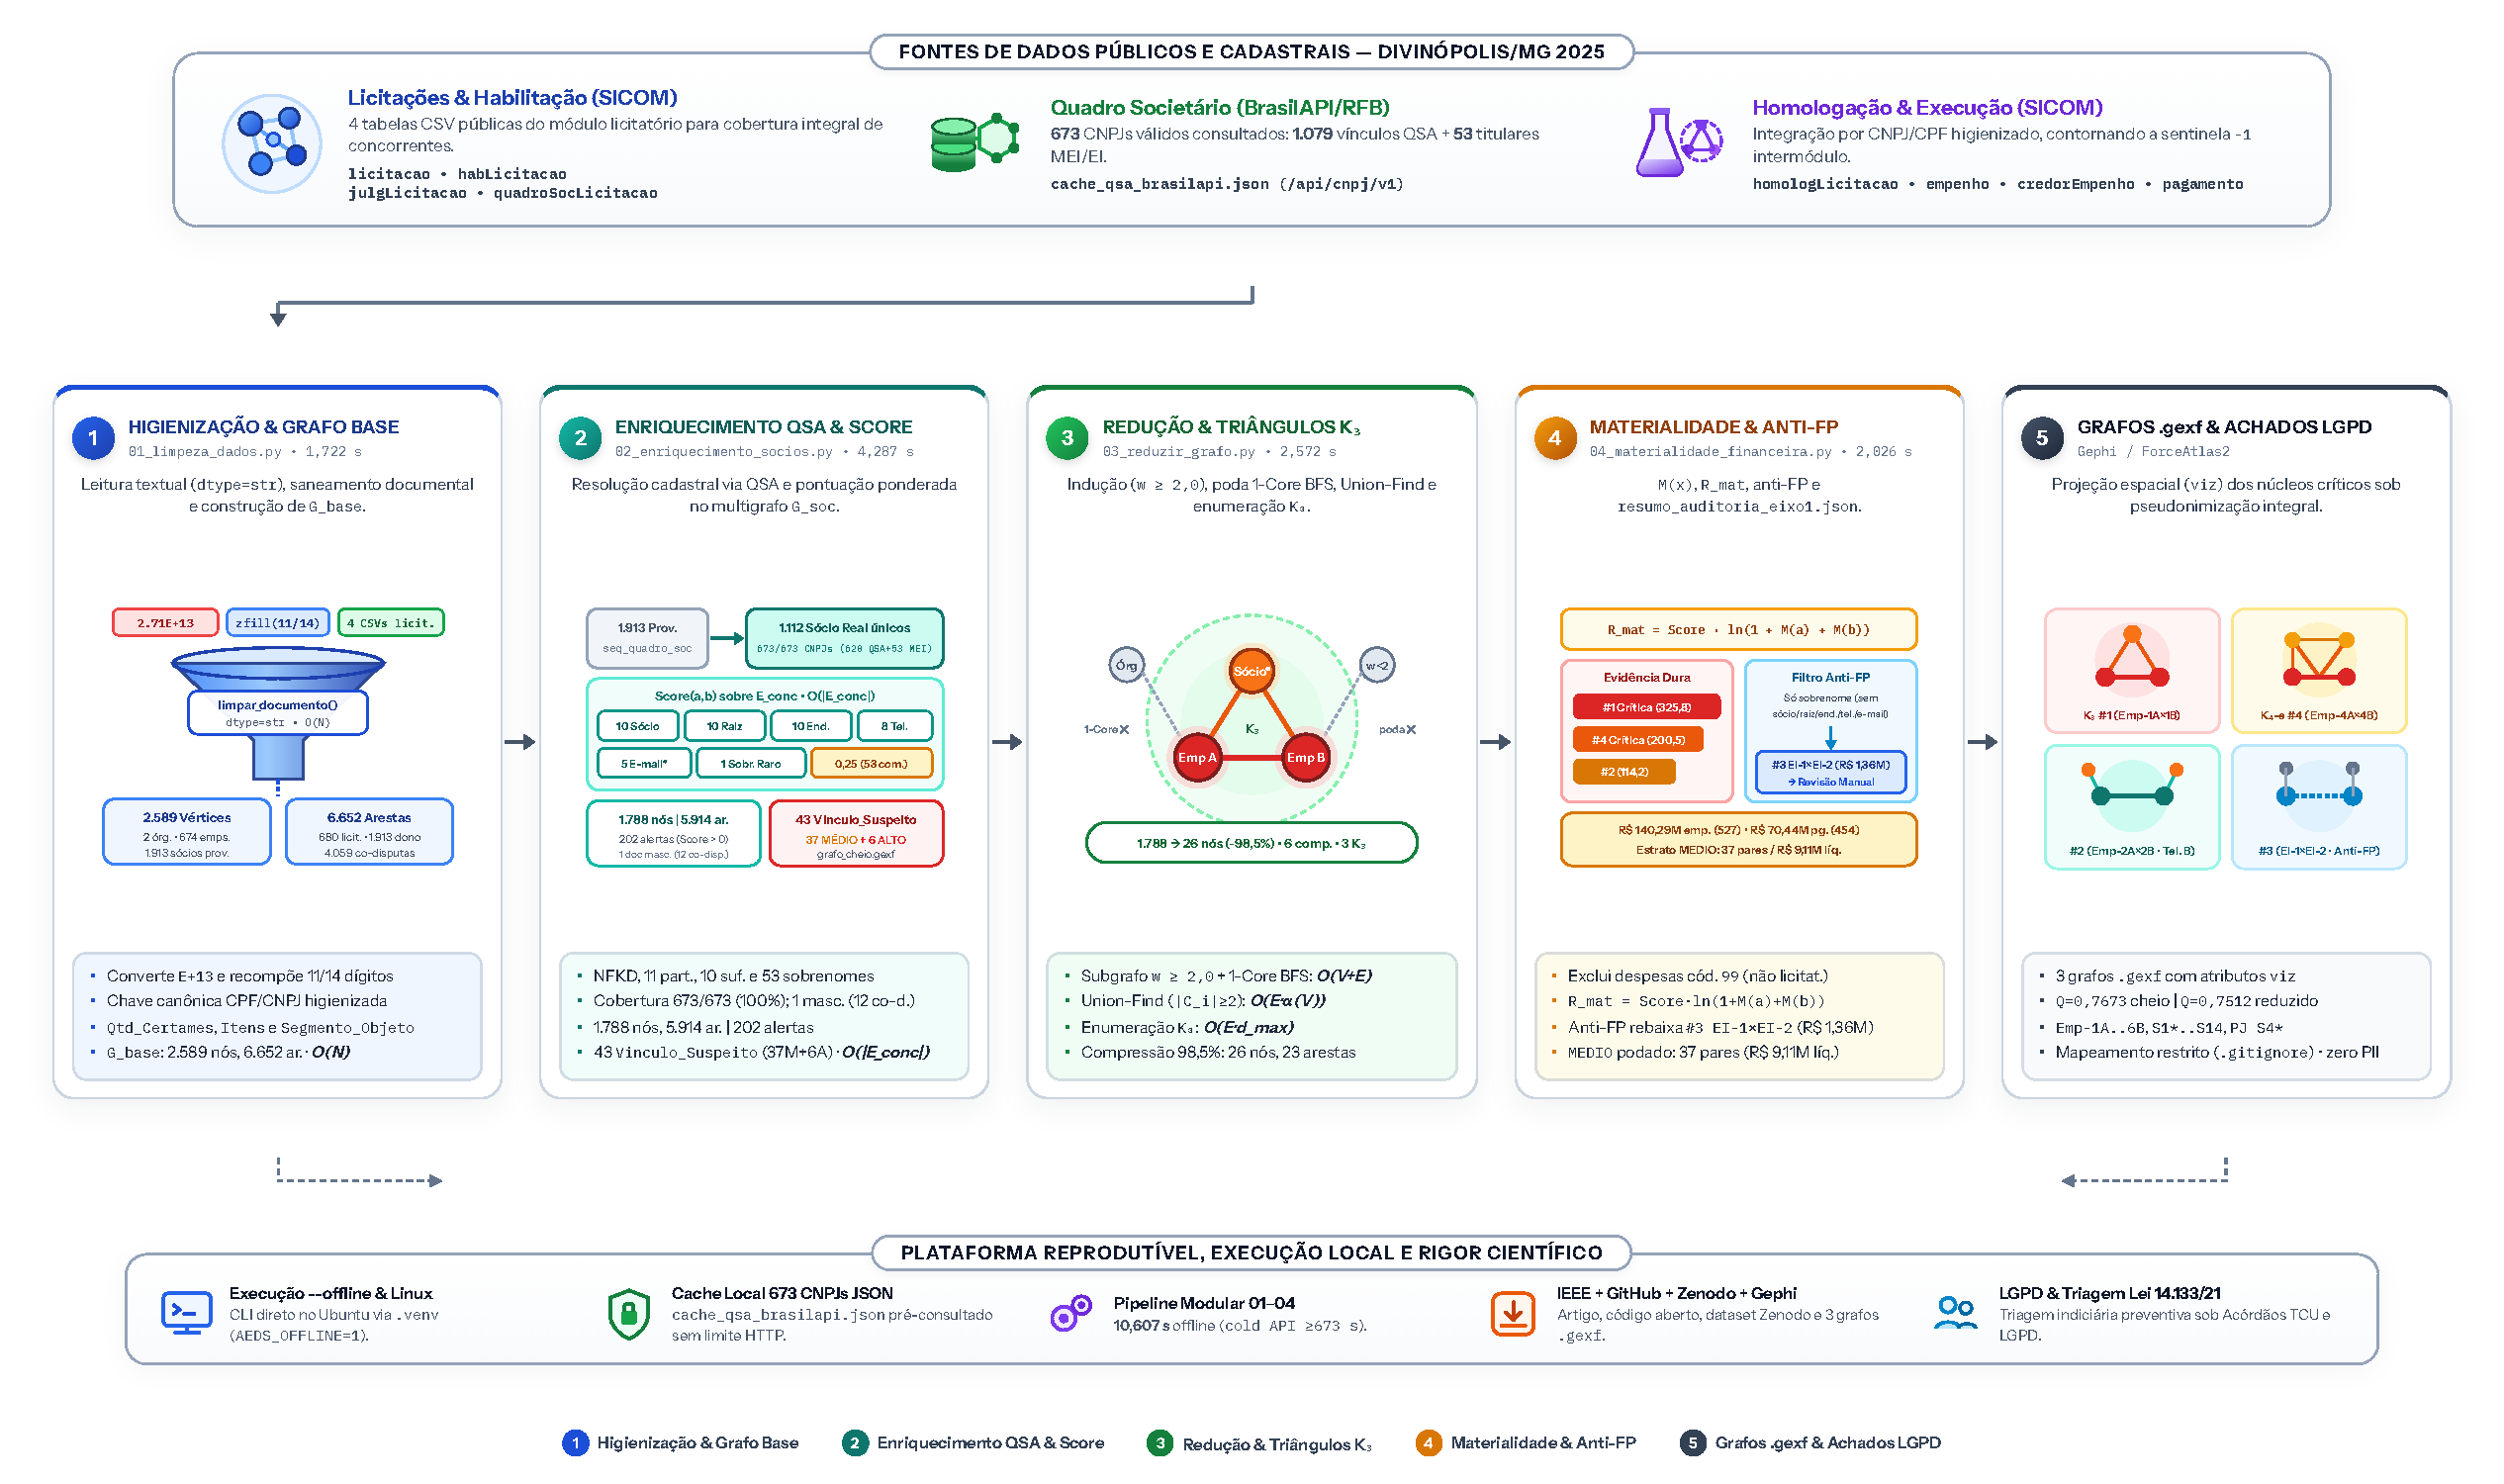
\includegraphics[width=0.93\textwidth]{figures/fluxograma_eixo1.pdf}
\caption{Fluxograma metodológico exclusivo do módulo \texttt{01\_\allowbreak analise\_\allowbreak socios}, organizando a camada superior de fontes públicas e cadastrais (SICOM/TCE-MG 2025 e BrasilAPI/RFB), os cinco blocos operacionais e visuais (1~Higienização \& Grafo Base, 2~Enriquecimento QSA \& Score, 3~Redução \& Triângulos $K_3$, 4~Materialidade \& Anti-FP e 5~Grafos \texttt{.gexf} \& Achados LGPD) com cobertura de 673/673 CNPJs, estrato \texttt{MEDIO} (R\$\,9,11\,M líq.), 10,607\,s em memória e governança LGPD com mapeamento restrito.}
\label{fig:fluxograma_eixo1}
\end{figure*}

\subsection{Obtenção e Tratamento de Dados}

Os registros licitatórios e financeiros provêm das remessas consolidadas de 2025 do município de Divinópolis/MG (código IBGE/SICOM \texttt{3122306}) no Portal de Dados Abertos do TCE-MG~\cite{tce_mg_dados_abertos,tcemg2025in01}. 
Foram processadas quatro tabelas relacionais em CSV delimitados por ponto e vírgula do módulo \texttt{licitacao} (\texttt{licitacao\allowbreak .csv}, \texttt{hab\allowbreak Licitacao\allowbreak .csv}, \texttt{julg\allowbreak Licitacao\allowbreak .csv} e \texttt{quadro\allowbreak Soc\allowbreak Licitacao\allowbreak .csv}) na modelagem estrutural. % além de \texttt{homolog\allowbreak Licitacao\allowbreak .csv}, \texttt{empenho\allowbreak .csv}, \texttt{credor\allowbreak Empenho\allowbreak .csv} e \texttt{pagamento\allowbreak .csv} na etapa de materialidade.

A análise exploratória dos dados revelou um gargalo de integridade na base pública: documentos fiscais (CPF/CNPJ) exportados em planilhas com perda de zeros à esquerda ou notação científica literal (ex.: \texttt{2.71E+13}).  %e (ii) preenchimento sistemático das chaves estrangeiras intermódulo (\texttt{seq\_\allowbreak licitacao} e \texttt{seq\_\allowbreak dispensa}) com o valor sentinela \texttt{-1} nas tabelas de contratos e empenhos, inviabilizando a junção direta entre um certame isolado e seu empenho correspondente. Em contrapartida, as chaves intramódulo (\texttt{seq\_\allowbreak licitacao}, \texttt{seq\_\allowbreak item\_\allowbreak licitacao} e \texttt{seq\_\allowbreak empenho}) preservam integridade completa, permitindo usar o documento fiscal higienizado como chave canônica de integração entre licitações e execução orçamentária.
Aplicou-se uma rotina de saneamento estrutural para corrigir mutações de formatação em notação científica  e restaurar os zeros à esquerda, padronizando 14 dígitos para pessoas jurídicas (CNPJ) e 11 dígitos para pessoas físicas (CPF). Em seguida, consolidoum-se os participantes únicos registrados nas fases de habilitação e julgamento dos certames.

\subsection{Modelagem do Grafo Multicamada}

%A partir da análise exploratória dos dados, todas as tabelas são carregadas em modo estritamente textual (\texttt{dtype=str}). Foram removidas pontuações, converção de expressões em notação científica (\texttt{E+}) para inteiro longo e recompoziação de zeros à esquerda para 11 dígitos (CPF) ou 14 dígitos (CNPJ). Na sequência, construiu-se o grafo base $G_{\text{base}}$:

Após consolidar o conjunto único de licitantes participantes nas fases de habilitação e julgamento, a malha de contratações públicas é formalmente modelada como um grafo heterogêneo multicamada ponderado \begin{equation} G = (V,E,\tau,\phi,w). \end{equation} Nessa formulação, $V$ denota o conjunto global de entidades e $E \subseteq V \times V$ representa o conjunto de interações. A heterogeneidade das entidades é definida pela função de mapeamento $\tau : V \rightarrow \mathcal{T}_V$, enquanto a estrutura multicamada é estabelecida pela função $\phi : E \rightarrow \mathcal{T}_E$, que segrega as relações em quatro camadas sobrepostas. Por fim, a função de ponderação $w : E \rightarrow \mathbb{R}^{+}$ associa a cada aresta uma métrica escalar de intensidade. \subsubsection{Partições de Vértices ($\mathcal{T}_V$)} \begin{itemize} \item \textbf{Órgãos Públicos ($\tau(v)=\text{Órgão}$):} representam as entidades contratantes da administração pública municipal. \item \textbf{Empresas Licitantes ($\tau(v)=\text{Empresa}$):} compreendem os agentes econômicos (pessoas jurídicas e físicas) participantes das fases de habilitação ou julgamento dos certames. \item \textbf{Sócios e Controladores ($\tau(v)=\text{Sócio Real}$):} correspondem aos proprietários e administradores vinculados às empresas licitantes, englobando tanto pessoas físicas (\texttt{PF}) quanto pessoas jurídicas ou \textit{holdings} (\texttt{PJ}). \end{itemize} \subsubsection{Camadas de Arestas ($\mathcal{T}_E$)} \begin{itemize} \item \texttt{Participou\_Licitacao}: camada bipartida que conecta cada \texttt{Empresa} ao respectivo \texttt{Órgão} contratante. \item \texttt{Concorreu\_Contra}: projeção ponderada monopartida entre pares de \texttt{Empresa} que disputaram os mesmos certames, cujo peso acumula a frequência absoluta de licitações e itens individuais disputados em comum. \item \texttt{É\_Dono\_De}: camada bipartida de propriedade que vincula cada \texttt{Sócio Real} às respectivas empresas (\texttt{Empresa}) integrantes de seu quadro societário. \item \texttt{Vinculo\_Suspeito}: camada indiciária filtrada entre pares concorrentes de \texttt{Empresa} que apresentam sobreposição cadastral, societária ou onomástica relevante, ponderada pelo escore de vínculo $w(e)=s(a,b)$. \end{itemize} Embora relações como \texttt{É\_Dono\_De} e \texttt{Participou\_Licitacao} possuam direcionalidade semântica natural, todas as arestas são armazenadas de forma simétrica (não-direcionada) na estrutura computacional em lista de adjacência, viabilizando a poda de grau e a detecção direta de ciclos fechados envolvendo empresas concorrentes e seus controladores em comum.

\subsection{Enriquecimento Societário e Escore Multidimensional de Vínculo} 

Como a tabela societária original do SICOM suprime nomes e CPFs dos sócios por restrição cadastral, executou-se um enriquecimento dos dados mediante consultas automatizadas ao Quadro de Sócios e Administradores (QSA) da Receita Federal via BrasilAPI para os CNPJs licitantes, com persistência em cache local. Para Microempreendedores Individuais (MEIs) e empresários individuais desprovidos de QSA formal, o titular é extraído diretamente da razão social mediante a remoção dos dígitos iniciais do documento. Para evitar falsos positivos decorrentes de dados cadastrais incompletos ou terceirização contábil, aplicam-se filtros determinísticos anti-ruído antes das comparações entre pares: 
\begin{itemize} 
  \item \textbf{Endereços e Telefones:} normalizam-se logradouro, número, município e unidade federativa, descartando entradas genéricas ou sem número e exigindo sequências telefônicas válidas com ao menos oito dígitos. \item \textbf{Correio Eletrônico:} endereços contendo termos associados a escritórios terceirizados (\texttt{contabil}, \texttt{contador}, \texttt{contabilidade}, \texttt{assessoria} e \texttt{escritorio}) são descartados automaticamente. 
  \item \textbf{Onomástica (Sobrenomes):} consideram-se exclusivamente sócios pessoas físicas ou titulares de MEI, removendo o primeiro prenome, preposições conectoras e sufixos de agnação. 
\end{itemize} 
Para atenuar falsos positivos decorrentes de homonímia conuns brasileiras,implementou-se uma ponderação onomástica discreta inspirada no princípio da Frequência Inversa de Documentos (IDF). Cada sobrenome compartilhado $n$ recebe peso reduzido $w(n)=0,25$ quando pertence a um dicionário de sobrenomes triviais, e peso integral $w(n)=1,00$ caso contrário. Para cada par de empresas concorrentes $(a,b)$ conectado na camada \texttt{Concorreu\_Contra}, o escore de vínculo é definido por: \begin{equation} \begin{aligned} s(a,b) =\;& 10 \cdot |S(a)\cap S(b)| \\ & + 10\cdot[\mathrm{raiz}(a)=\mathrm{raiz}(b)] \\ & + 10\cdot[\mathrm{end}(a)=\mathrm{end}(b)] \\ & + 8\cdot[\mathrm{tel}(a)=\mathrm{tel}(b)] \\ & + 5\cdot[\mathrm{email}(a)=\mathrm{email}(b)] \\ & + \sum_{n\in N(a)\cap N(b)} w(n). \end{aligned} \end{equation} onde $S(x)$ denota o conjunto de sócios da empresa $x$, $\mathrm{raiz}(x)$ os oito primeiros dígitos do CNPJ, $\mathrm{end}(x)$, $\mathrm{tel}(x)$ e $\mathrm{email}(x)$ os atributos cadastrais higienizados, e $N(x)$ o conjunto de sobrenomes extraídos. A recorrência acumulada de disputas (\texttt{Peso\_Concorrencia}) não integra a soma de $s(a,b)$, sendo utilizada exclusivamente como critério de desempate na ordenação dos alertas. Os pares com $s(a,b)>0$ são estratificados em três níveis de criticidade: \texttt{ALTO}, quando há identidade direta de sócio, raiz de CNPJ, endereço ou telefone, ou quando $s(a,b)\geq 2,00$; \texttt{MEDIO}, quando $1,00 \leq s(a,b) < 2,00$ sem coincidência cadastral direta; e \texttt{BAIXO}, quando $0 < s(a,b) < 1,00$, sendo estes últimos omitidos da camada indiciária do grafo completo.

\subsection{Redução Topológica e Identificação de Motivos Estruturais ($K_3$)} 
Na rede completa, a elevada centralidade dos órgãos públicos e a densidade da concorrência regular ofuscam as estruturas de conluio. Para isolar os núcleos críticos, aplicou-se uma cadeia sequencial de quatro algoritmos formais em grafos. 
\begin{enumerate} 
\item \textbf{Subgrafo Induzido por Arestas (\textit{Edge-Induced Subgraph}):} Seja $V_{\text{suspeito}}$ o conjunto das empresas incidentes em alguma aresta \texttt{Vinculo\_Suspeito} com peso acima do limiar crítico $\theta = 2,00$. Em varredura linear de complexidade $O(|V|+|E|)$, retêm-se exclusivamente as arestas que satisfazem \begin{equation} \begin{aligned} \mathcal{P}(u,v,\mathrm{tipo},\mathrm{peso}) \iff &\;(\mathrm{tipo}=\texttt{Vinculo\_Suspeito} \\ &\land \mathrm{peso}\geq\theta) \\ &\lor (\mathrm{tipo}=\texttt{É\_Dono\_De} \\ &\land (u\in V_{\text{suspeito}} \lor v\in V_{\text{suspeito}})). \end{aligned} \end{equation} \
\item \textbf{Decomposição 1-Core via BFS:} Utilizando uma fila FIFO (\textit{First-In, First-Out}), executa-se a poda iterativa de grau em complexidade $O(|V|+|E|)$, removendo todos os vértices com grau $d(u)<1$ e preservando exclusivamente os nós ativos no subgrafo reduzido. \item \textbf{Componentes Conexas via Union-Find:} Aplica-se a estrutura de conjuntos disjuntos (\textit{Disjoint Set}) otimizada com \textit{path compression} e \textit{union by rank}, resultando em complexidade quase linear \begin{equation} O(|E| \cdot \alpha(|V|)), \end{equation} onde $\alpha$ representa a função inversa de Ackermann. Retendo apenas componentes não triviais ($|C_i| \geq 2$), a rede é particionada em núcleos independentes de suspeita para auditoria. \item \textbf{Listagem de Triângulos Societários (\textit{Triangle Listing} -- Motivo $K_3$):} Para detectar ciclos fechados de controle econômico compartilhado ($\text{Sócio} - E_1 - E_2 - \text{Sócio}$), constrói-se o mapeamento \begin{equation} \mathrm{donos}[e] = \{s \mid (s,e)\in E_{\texttt{É\_Dono\_De}}\}, \end{equation} e calcula-se a interseção \begin{equation} \mathrm{donos}[e_1]\cap \mathrm{donos}[e_2] \end{equation} para cada aresta suspeita $(e_1,e_2)$ em tempo $O(|E|\cdot d_{\max})$, sendo $d_{\max}$ o número máximo de sócios por empresa. A presença do motivo estrutural $K_3$ formaliza a evidência topológica de ausência de independência decisória entre licitantes formalmente concorrentes. \end{enumerate}

\subsection{Conformidade com a LGPD e Ética em Pesquisa Pública}

Embora as remessas do SICOM/TCE-MG e os dados cadastrais do QSA sejam públicos por determinação legal, a divulgação acadêmica de escores de risco exige proteção proporcional de pessoas naturais e jurídicas conforme a LGPD~\cite{brasil2018lgpd} e os parâmetros do TCU~\cite{tcu2011acordao2341,tcu2024acordao1798}. Em observância à minimização e à adequação de finalidade (art.~6º, incisos~I a III), todo o texto, as tabelas e as figuras aplicam pseudonimização integral: os 14 vértices de sócio dos núcleos reduzidos recebem códigos \texttt{S1*}--\texttt{S14} (sendo \texttt{PJ S4*} uma pessoa jurídica sócia e o sufixo \texttt{*} reservado aos sócios-ponte que fecham triângulos $K_3$), os endereços e telefones coincidentes constam como \texttt{End.~A/B} e \texttt{Tel.~A/B}, as empresas privadas e empresários individuais recebem rótulos \texttt{Emp-1A}--\texttt{Emp-6B} e \texttt{EI-1}--\texttt{EI-2}, e suprimem-se integralmente CPFs, CNPJs e nomes civis. % Para permitir auditoria externa pelas autoridades competentes sem expor dados pessoais no artigo ou no repositório público, a Etapa~4 gera localmente a chave de reversão \texttt{mapeamento\_\allowbreak pseudonimos\_\allowbreak restrito\allowbreak .csv} (30 registros), mantida estritamente offline sob proteção de \texttt{.gitignore}.

\section{Resultados e Discussão}
\label{sec:resultados}

A execução integral da abordagem metodológica sobre as bases consolidadas de Divinópolis/MG em 2025 demonstrou capacidade de compressão estrutural e separação entre riscos críticos, passivos inativos e falsos positivos onomásticos. Em observância ao protocolo ético e à LGPD, todos os atores privados e sócios são designados exclusivamente por seus pseudônimos oficiais.

\begin{figure*}[!t]
\centering
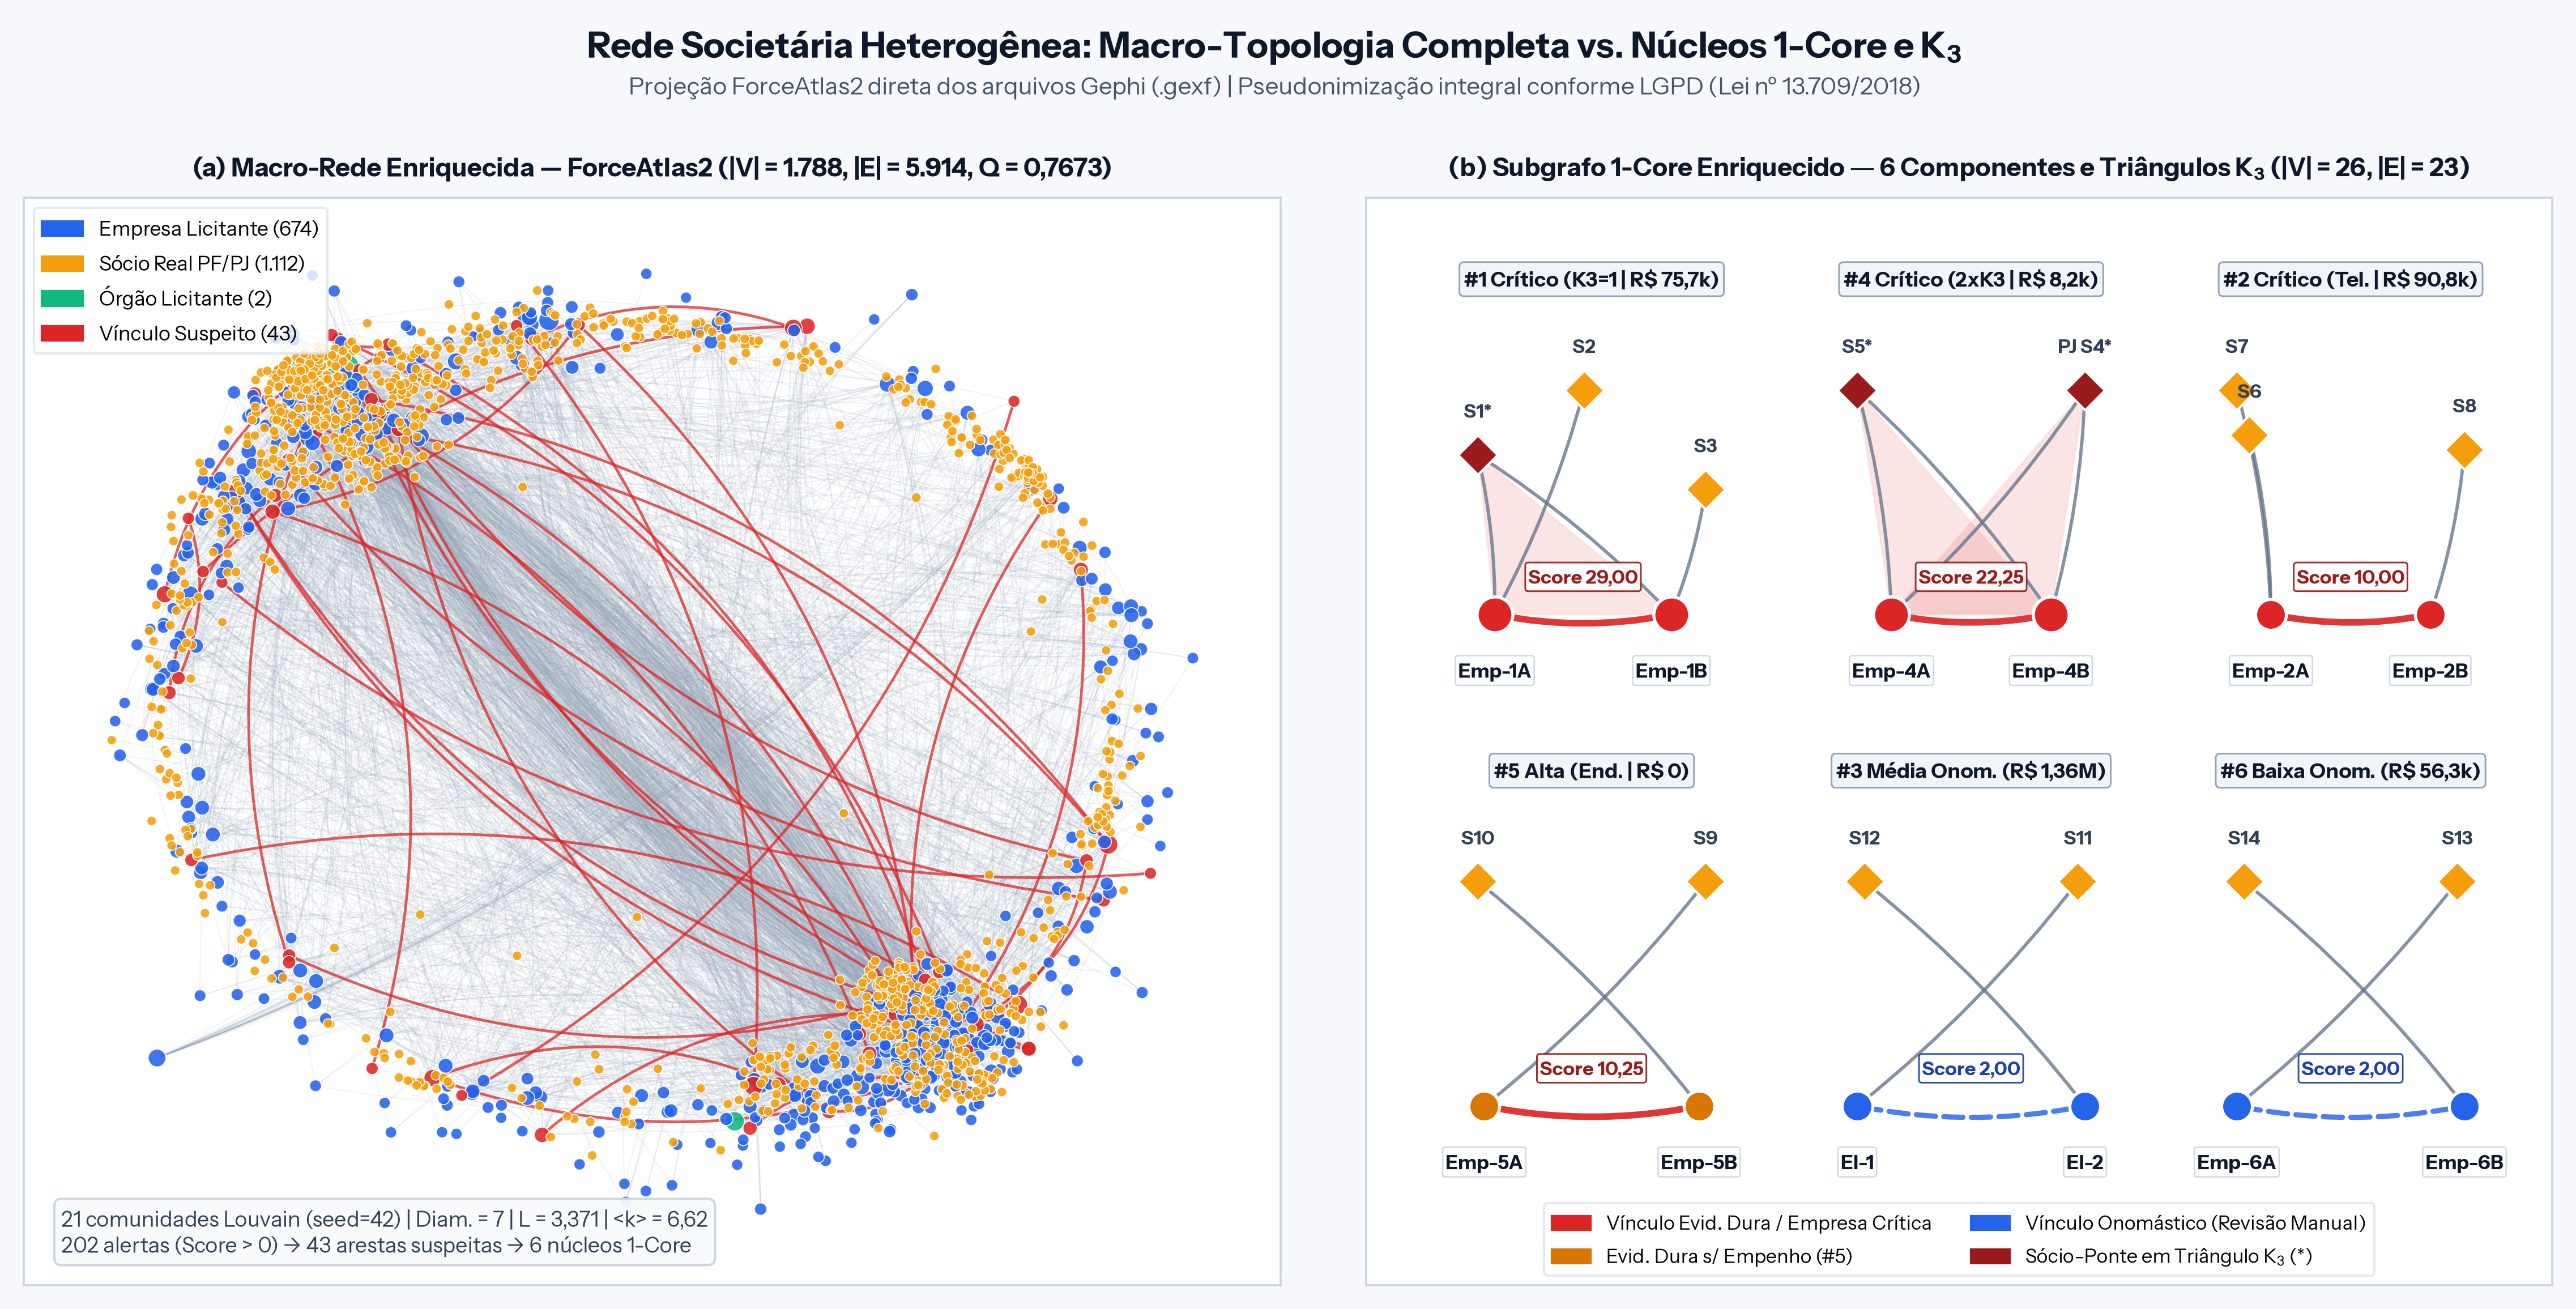
\includegraphics[width=0.72\textwidth]{figures/eixo1_rede_societaria_k3.png}
\caption{Visualização ForceAtlas2 dos grafos Gephi (\texttt{.gexf}) do módulo \texttt{01\_\allowbreak analise\_\allowbreak socios}: (a) macro-rede enriquecida (\texttt{grafo\_\allowbreak cheio.gexf}, $|V|=1.788$, $|E|=5.914$, $Q=0{,}7673$, 21 comunidades Louvain) destacando as 43 arestas \textnormal{\textit{Vinculo\_\allowbreak Suspeito}} (37 \texttt{MEDIO} e 6 \texttt{ALTO}, plotadas em vermelho no painel e diferenciadas entre âmbar e vermelho no \texttt{.gexf}); e (b) subgrafo $1$-core enriquecido (\texttt{subgrafos\_\allowbreak fraudes\_\allowbreak enriquecido.gexf}, $|V|=26$, $|E|=23$) exibindo os 6 componentes e triângulos $K_3$ sombreados (\#1 e \#4).}
\label{fig:eixo1_rede}
\end{figure*}

\subsection{Evolução Estrutural ao Longo das Quatro Etapas}

Na Etapa~1 (\texttt{01\_\allowbreak limpeza\_\allowbreak dados.py}), o saneamento documental produziu um grafo base de \textbf{2.589 vértices} (2 órgãos licitantes — Executivo \texttt{Orgao\_02} e Legislativo \texttt{Orgao\_01} —, 674 empresas licitantes e 1.913 registros provisórios \texttt{seq\_\allowbreak quadro\_\allowbreak soc}) e \textbf{6.652 arestas} (4.059 de \textit{Concorreu\_\allowbreak Contra}, 1.913 de \textit{É\_\allowbreak Dono\_\allowbreak De} e 680 de \textit{Participou\_\allowbreak Licitacao}). Dos 674 documentos licitantes, 673 correspondiam a CNPJs válidos de 14 dígitos e 1 constituía registro mascarado na base pública, cuja participação representou 13 arestas no grafo cheio (12 de \textit{Concorreu\_\allowbreak Contra} e 1 de \textit{Participou\_\allowbreak Licitacao}), 0 itens homologados e 2 empenhos somando R\$\,4.620,00 líquidos (R\$\,0,00 pagos).

Na Etapa~2 (\texttt{02\_\allowbreak enriquecimento\_\allowbreak socios.py}), a resolução cadastral via BrasilAPI atingiu \textbf{100,0\% de cobertura sobre os 673 CNPJs válidos} (\textbf{620} com QSA da Receita Federal e \textbf{53} titulares MEI/EI extraídos da razão social, zero vazios ou erros), recuperando \textbf{1.132 vínculos societários válidos} (1.079 QSA + 53 MEI/EI) e consolidando homônimos sequenciais em \textbf{1.112 vértices \textit{Sócio Real}} únicos. Substituindo os nós provisórios e incorporando as 43 arestas suspeitas paralelas (37 de nível \texttt{MEDIO} e 6 de nível \texttt{ALTO}), o grafo cheio (\texttt{grafo\_\allowbreak cheio.gexf}) alcançou \textbf{1.788 vértices} e \textbf{5.914 arestas}, formando uma única componente conexa ($\text{WCC}=1$, diâmetro 7, distância geodésica média $L=3{,}371$) organizada no multigrafo em 21 comunidades de Louvain (\texttt{seed=42}) com elevada modularidade ($Q=0{,}7673$).

O cômputo de escores sobre os 4.059 pares co-disputantes gerou exatamente \textbf{202 alertas com $\text{Score} > 0$}, cuja distribuição empírica consta na Figura~\ref{fig:eixo1_metricas}~(a). Verifica-se que \textbf{159 pares (78,7\%)} enquadram-se no nível \texttt{BAIXO} ($\text{Score}=0{,}25$ em 156 casos e $0{,}50$ em 3 casos, decorrentes de um ou dois sobrenomes frequentes) e \textbf{37 pares (18,3\%)} compõem o nível \texttt{MEDIO} ($\text{Score}=1{,}00$ em 34 casos e $1{,}25$ em 3 casos). Segundo \texttt{resumo\_\allowbreak auditoria\_\allowbreak eixo1\allowbreak .json}, esse estrato \texttt{MEDIO} podado pelo corte $w \ge 2{,}0$ envolve \textbf{61 empresas distintas} (30 pares com empenho bilateral, 4 com unilateral e 3 sem empenho), acumulando \textbf{R\$\,11.342.332,96} em soma par a par ou \textbf{R\$\,9.114.055,59} líquidos em empresas distintas (R\$\,444.663,53 homologados e R\$\,6.474.916,37 pagos), preservado em \texttt{alertas\_\allowbreak vinculos\_\allowbreak concorrentes\allowbreak .csv} sem contaminar o subgrafo crítico. Apenas \textbf{6 pares (3,0\%)} atingiram o limiar de alto risco ($\text{Score} \ge 2{,}0$), concentrando integralmente as coincidências objetivas detectadas no município: 2 pares com sócios em comum, 2 com mesmo endereço comercial, 2 com mesmo telefone corporativo, nenhum par com e-mail compartilhado (após filtragem de escritórios contábeis) e nenhum par com mesma raiz de CNPJ.

Na Etapa~3 (\texttt{03\_\allowbreak reduzir\_\allowbreak grafo.py}), a cadeia determinística de indução ($w \ge 2{,}0$, descartando as 37 arestas \texttt{MEDIO} e retendo apenas as 6 arestas \texttt{ALTO}), poda $1$-core via BFS e Union-Find comprimiu os 1.788 vértices da macro-rede para apenas \textbf{26 vértices} (12 empresas e 14 sócios) e \textbf{23 arestas} (6 arestas \textit{Vinculo\_\allowbreak Suspeito} e 17 arestas \textit{É\_\allowbreak Dono\_\allowbreak De}), reduzindo em \textbf{98,5\%} a cardinalidade de vértices auditados. Esse corte isolou \textbf{6 componentes conexos} independentes e enumerou \textbf{3 triângulos societários fechados ($K_3$)}, conforme ilustrado na projeção \textit{ForceAtlas2} da Figura~\ref{fig:eixo1_rede}.

\subsection{Anatomia dos Seis Componentes, Triângulos $K_3$ e Materialidade}

Na Etapa~4 (\texttt{04\_\allowbreak materialidade\_\allowbreak financeira.py}), o cruzamento por CNPJ/CPF higienizado abrangeu todas as 674 empresas do grafo base: apenas 88 apresentaram valor homologado positivo em \texttt{homolog\allowbreak Licitacao\allowbreak .csv} (somando R\$\,25.771.978,02 em 929 itens homologados), ao passo que \textbf{527 empresas} registraram empenhos contratuais líquidos positivos em 2025 (totalizando \textbf{R\$\,140.293.315,49}, dos quais R\$\,70.440.903,07 foram pagos a 454 credores). A Figura~\ref{fig:eixo1_componentes} expõe a topologia individual dos seis núcleos reduzidos, enquanto a Tabela~\ref{tab:eixo1_ranking} apresenta o \textit{ranking} completo de priorização.

\begin{figure*}[!t]
\centering
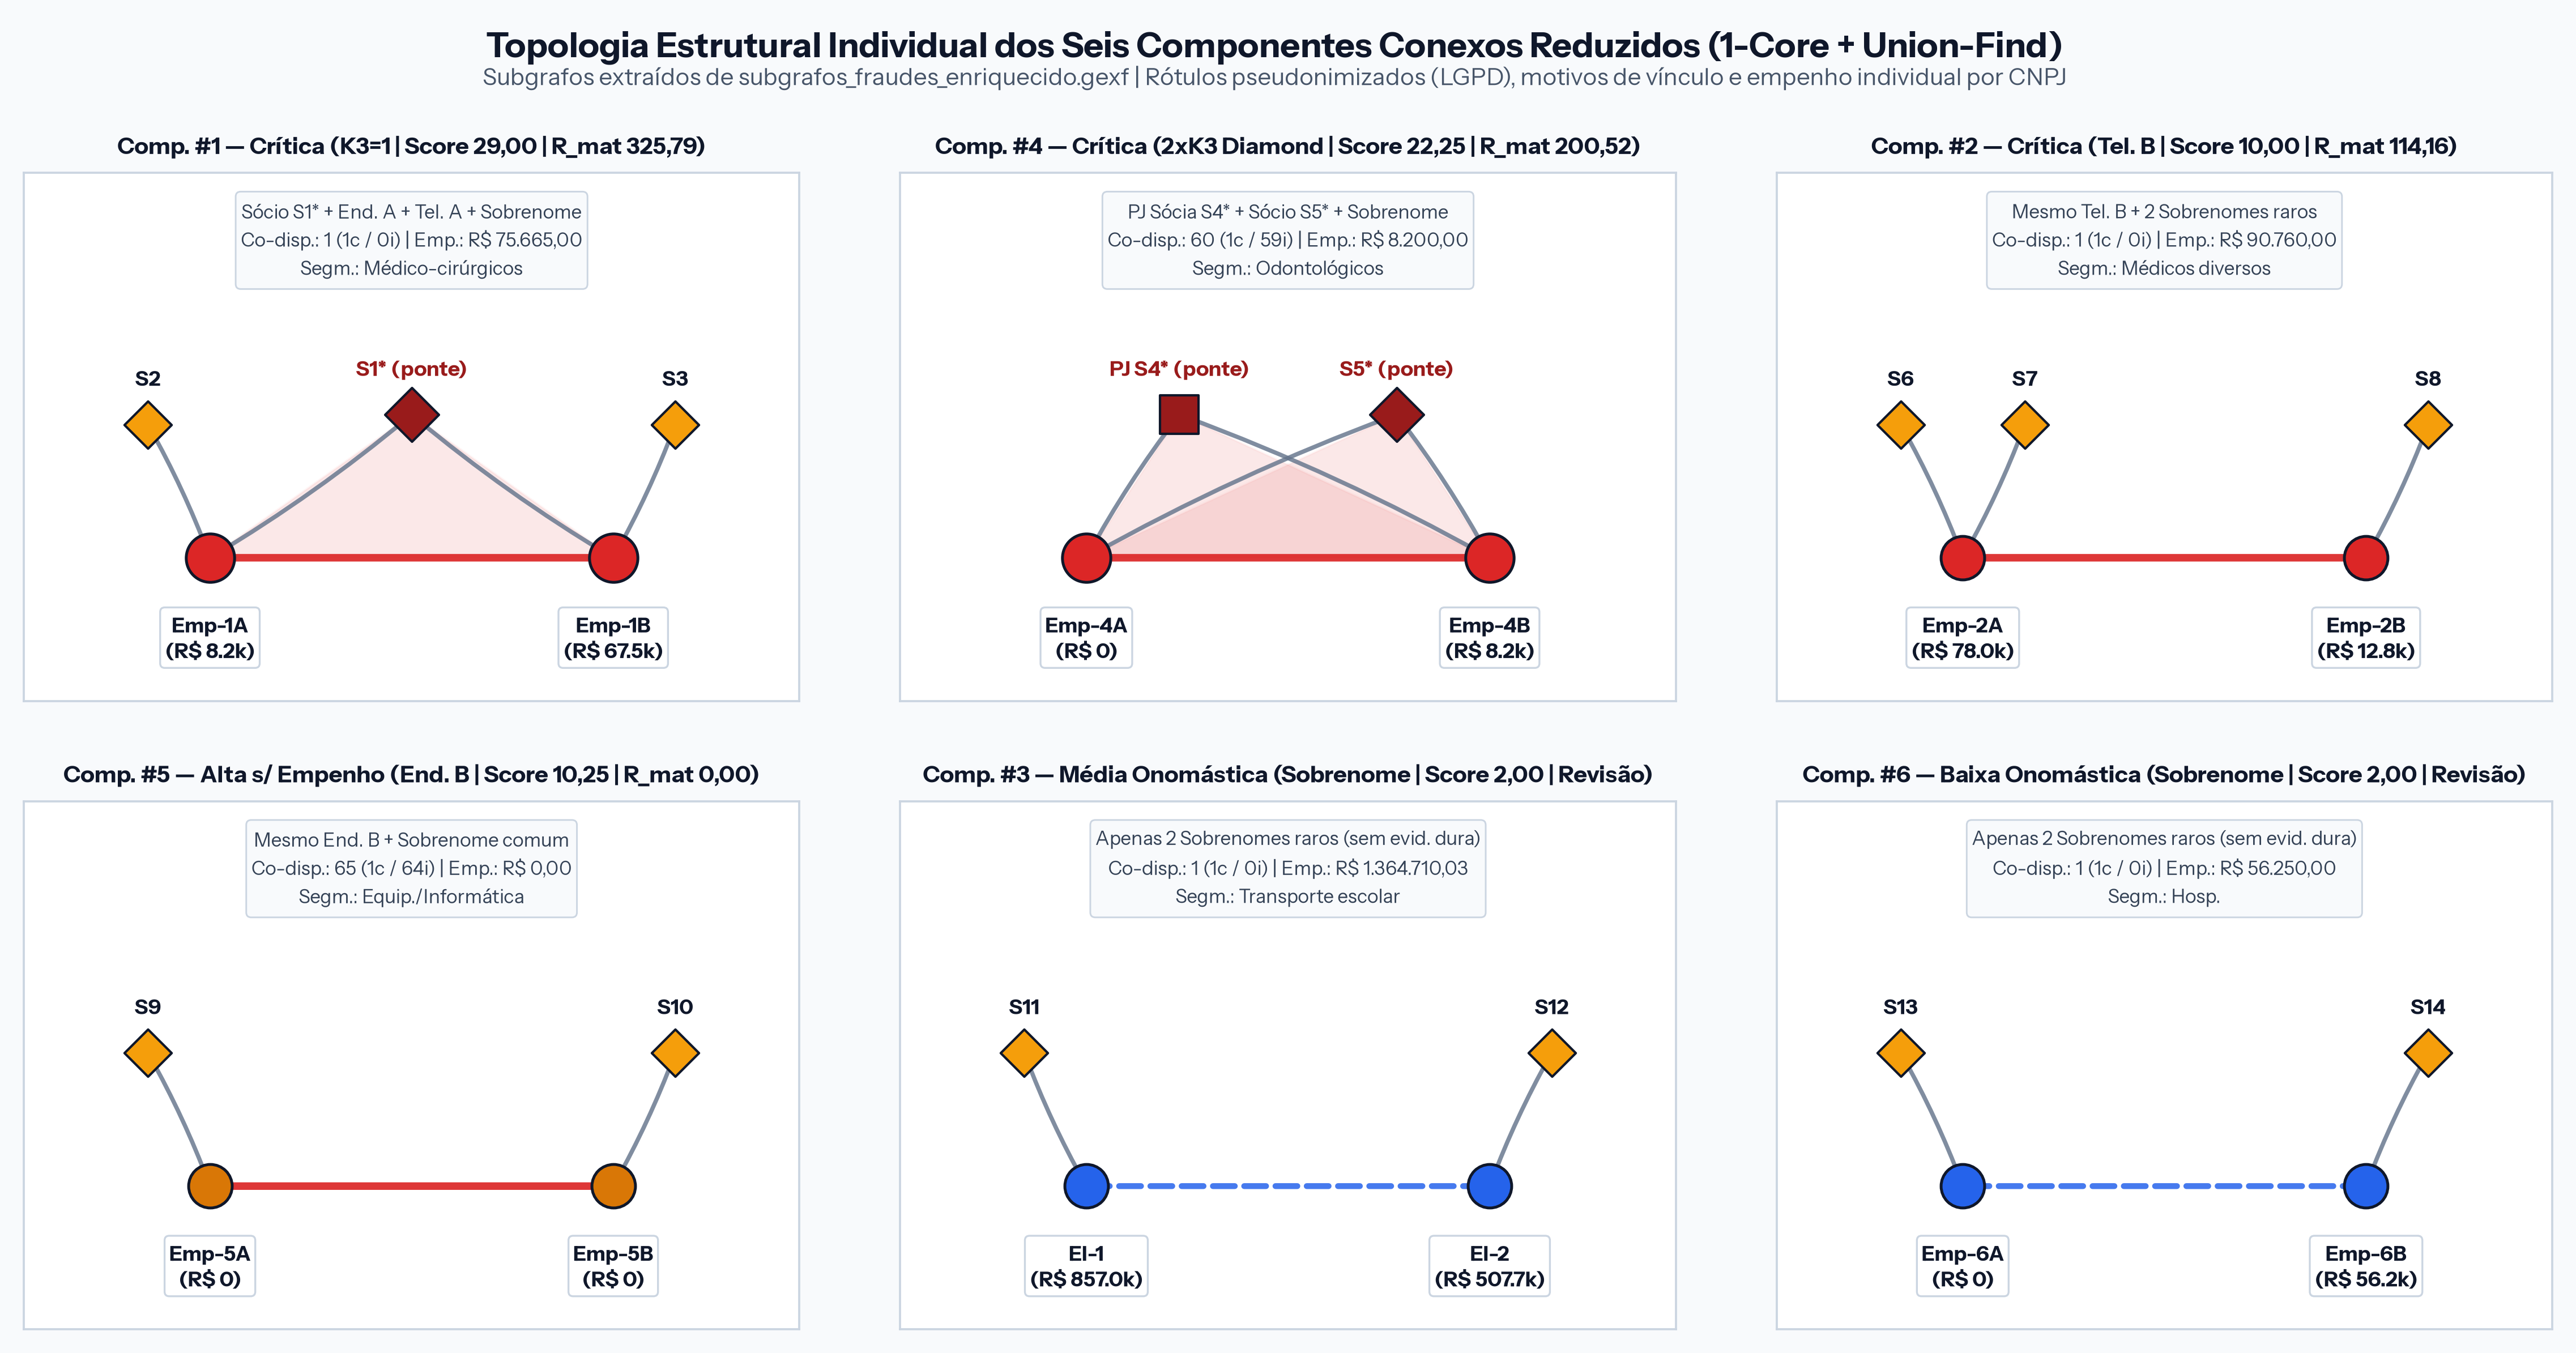
\includegraphics[width=0.71\textwidth]{figures/eixo1_componentes_detalhados.png}
\caption{Inspeção estrutural individual dos seis componentes conexos em \texttt{subgrafos\_\allowbreak fraudes\_\allowbreak enriquecido.gexf}, detalhando os triângulos $K_3$ simples (\#1) e duplo/diamante $K_4-e$ (\#4), cadeias acíclicas por telefone/endereço (\#2 e \#5), falsos positivos onomásticos (\#3 e \#6), decomposição de co-disputas (\textit{certames/itens}), segmento de objeto e empenho líquido por CNPJ sob pseudonimização LGPD.}
\label{fig:eixo1_componentes}
\end{figure*}

\begin{table*}[!t]
\centering
\caption{Ranking de priorização dos seis componentes conexos após cruzamento financeiro e filtro anti-falso positivo.}
\label{tab:eixo1_ranking}
\resizebox{\textwidth}{!}{%
\begin{tabular}{@{}clccllrrrrl@{}}
\toprule
\textbf{Comp.} & \textbf{Par Concorrente} & \textbf{Cert. / Itens} & \textbf{Score} & \textbf{Segmento} & \textbf{Critérios / Padrão Topológico} & \textbf{Empenhado Líq.} & \textbf{Pago Líq.} & \textbf{Risco Mat.} & \textbf{Classificação Final} \\
\midrule
\#1 & \texttt{Emp-1A} $\times$ \texttt{Emp-1B} & 1c / 0i & 29,00 & Médico-cirúrgicos & \texttt{S1*}, \texttt{End. A}, \texttt{Tel. A} ($K_3=1$) & R\$\,75.665,00 & R\$\,64.120,00 & 325,79 & Crítica (Evid. Dura + Contrato) \\
\#4 & \texttt{Emp-4A} $\times$ \texttt{Emp-4B} & 1c / 59i & 22,25 & Odontológicos & \texttt{PJ S4*}, \texttt{S5*} ($2\times K_3$, $K_4-e$) & R\$\,8.200,00 & R\$\,8.200,00 & 200,52 & Crítica (Evid. Dura + Contrato) \\
\#2 & \texttt{Emp-2A} $\times$ \texttt{Emp-2B} & 1c / 0i & 10,00 & Médicos diversos & \texttt{Tel. B}, 2 sobr. raros (árvore) & R\$\,90.760,00 & R\$\,87.200,00 & 114,16 & Crítica (Evid. Dura + Contrato) \\
\#5 & \texttt{Emp-5A} $\times$ \texttt{Emp-5B} & 1c / 64i & 10,25 & Equip./Informática & \texttt{End. B}, sobr. comum ($P_4$) & R\$\,0,00 & R\$\,0,00 & 0,00 & Alta (Evid. Dura s/ Empenho) \\
\#3 & \texttt{EI-1} $\times$ \texttt{EI-2} & 1c / 0i & 2,00 & Transporte escolar & Apenas 2 sobr. raros ($P_4$) & R\$\,1.364.710,03 & R\$\,819.965,10 & 28,25 & Média Onomástica (Rev. Manual) \\
\#6 & \texttt{Emp-6A} $\times$ \texttt{Emp-6B} & 1c / 0i & 2,00 & Hosp. & Apenas 2 sobr. raros ($P_4$) & R\$\,56.250,00 & R\$\,44.550,00 & 21,88 & Baixa Onomástica (Rev. Manual) \\
\bottomrule
\end{tabular}%
}
\end{table*}

Uma discussão crítica dos números da Tabela~\ref{tab:eixo1_ranking} revela dois aspectos metodológicos essenciais que explicam o comportamento do modelo:
\begin{enumerate}
  \item \textbf{Divergência entre homologações e empenhos} (\texttt{Vlr\_\allowbreak Homologado} nulo): nos seis componentes reduzidos, nenhuma das 12 empresas figurou como vencedora nos 929 registros de \texttt{homolog\allowbreak Licitacao\allowbreak .csv} de 2025, embora 5 componentes tenham movimentado empenhos contratuais expressivos. Esse fenômeno decorre do fato de que \texttt{homolog\allowbreak Licitacao\allowbreak .csv} cobre apenas 88 vencedores no exercício, deixando de fora empenhos oriundos de licitações homologadas em anos anteriores com execução continuada em 2025, adesões a atas e contratações diretas/dispensas não registradas na homologação licitatória. Caso a Etapa~4 dependesse exclusivamente das homologações do ano, todos os seis núcleos teriam materialidade nula; a regra de prioridade para \texttt{Vlr\_\allowbreak Empenhado\_\allowbreak Liq} garante cobertura efetiva da despesa contratada;
  \item \textbf{Rebaixamento consistente do Componente \#3 sem contradição:} embora o par \texttt{EI-1} $\times$ \texttt{EI-2} some R\$\,1.364.710,03 em 28 empenhos (\texttt{EI-1}: R\$\,856.966,20; \texttt{EI-2}: R\$\,507.743,83) e tenha atingido $\text{Score}=2{,}00$ pela coincidência de dois sobrenomes raros, o par não apresenta sócio em comum, mesma raiz CNPJ, endereço ou telefone (\texttt{Tem\_\allowbreak Evidencia\_\allowbreak Dura = False}). Em consonância com os Acórdãos do TCU~\cite{tcu2011acordao2341,tcu2024acordao1798}, a coincidência onomástica isolada — amplificada em bases de MEI/EI nas quais a Receita Federal não divulga o CPF do titular — não autoriza presunção de grupo econômico. O filtro da Etapa~4 preserva a rastreabilidade financeira (\texttt{MEDIA\_\allowbreak ONOMASTICA\_\allowbreak ALTA\_\allowbreak MATERIALIDADE} com \texttt{Validacao\_\allowbreak Manual = True}), posicionando \#3 ($R_{\text{mat}}=28{,}25$) abaixo dos três núcleos com evidência objetiva confirmada.
\end{enumerate}

\begin{table*}[!t]
\centering
\caption{Comparação topológica direta dos artefatos GEXF exportados para o Gephi no módulo \textnormal{\texttt{01\_\allowbreak analise\_\allowbreak socios}}.}
\label{tab:eixo1_gephi}
\resizebox{\textwidth}{!}{%
\begin{tabular}{@{}llrrrrrrrrr@{}}
\toprule
\textbf{Artefato (\texttt{.gexf})} & \textbf{Tipo} & \textbf{$|V|$} & \textbf{$|E|$} & \textbf{Densidade} & \textbf{$\langle k \rangle$} & \textbf{$\langle k_w \rangle$} & \textbf{$k_{\max}$} & \textbf{WCC (LCC)} & \textbf{$Q$ (Com. Louvain)} & \textbf{Diam. / $L$ (LCC)} \\
\midrule
\texttt{grafo\_cheio.gexf} (Etapa~2) & MultiGraph & 1.788 & 5.914 & 0,00370 & 6,62 & 80,06 & 628 & 1 (1.788) & 0,7673 (21) & 7 / 3,371 \\
\texttt{subgrafos\_fraudes.gexf} (Etapa~3) & Graph & 26 & 23 & 0,07077 & 1,77 & 7,12 & 3 & 6 (5) & 0,7512 (6) & 3 / 1,600 \\
\texttt{subgrafos\_fraudes\_enriquecido.gexf} (Etapa~4) & Graph & 26 & 23 & 0,07077 & 1,77 & 7,12 & 3 & 6 (5) & 0,7512 (6) & 3 / 1,600 \\
\bottomrule
\end{tabular}%
}
\par\vspace{2pt}{\footnotesize Notas: densidade e partição de Louvain (\texttt{seed=42}) computadas diretamente sobre o objeto NetworkX de cada \texttt{.gexf}; diâmetro e distância média $L$ avaliados na maior componente simples (LCC — nos subgrafos reduzidos, refere-se ao \texttt{Comp.~\#1} de 5 vértices; \texttt{Comp.~\#2}, também com 5 vértices, apresenta $L=1{,}800$, e a média global nos 44 pares conectados é $1{,}614$); $\langle k_w \rangle$ indica o grau médio ponderado.}
\end{table*}

\begin{figure*}[!t]
\centering
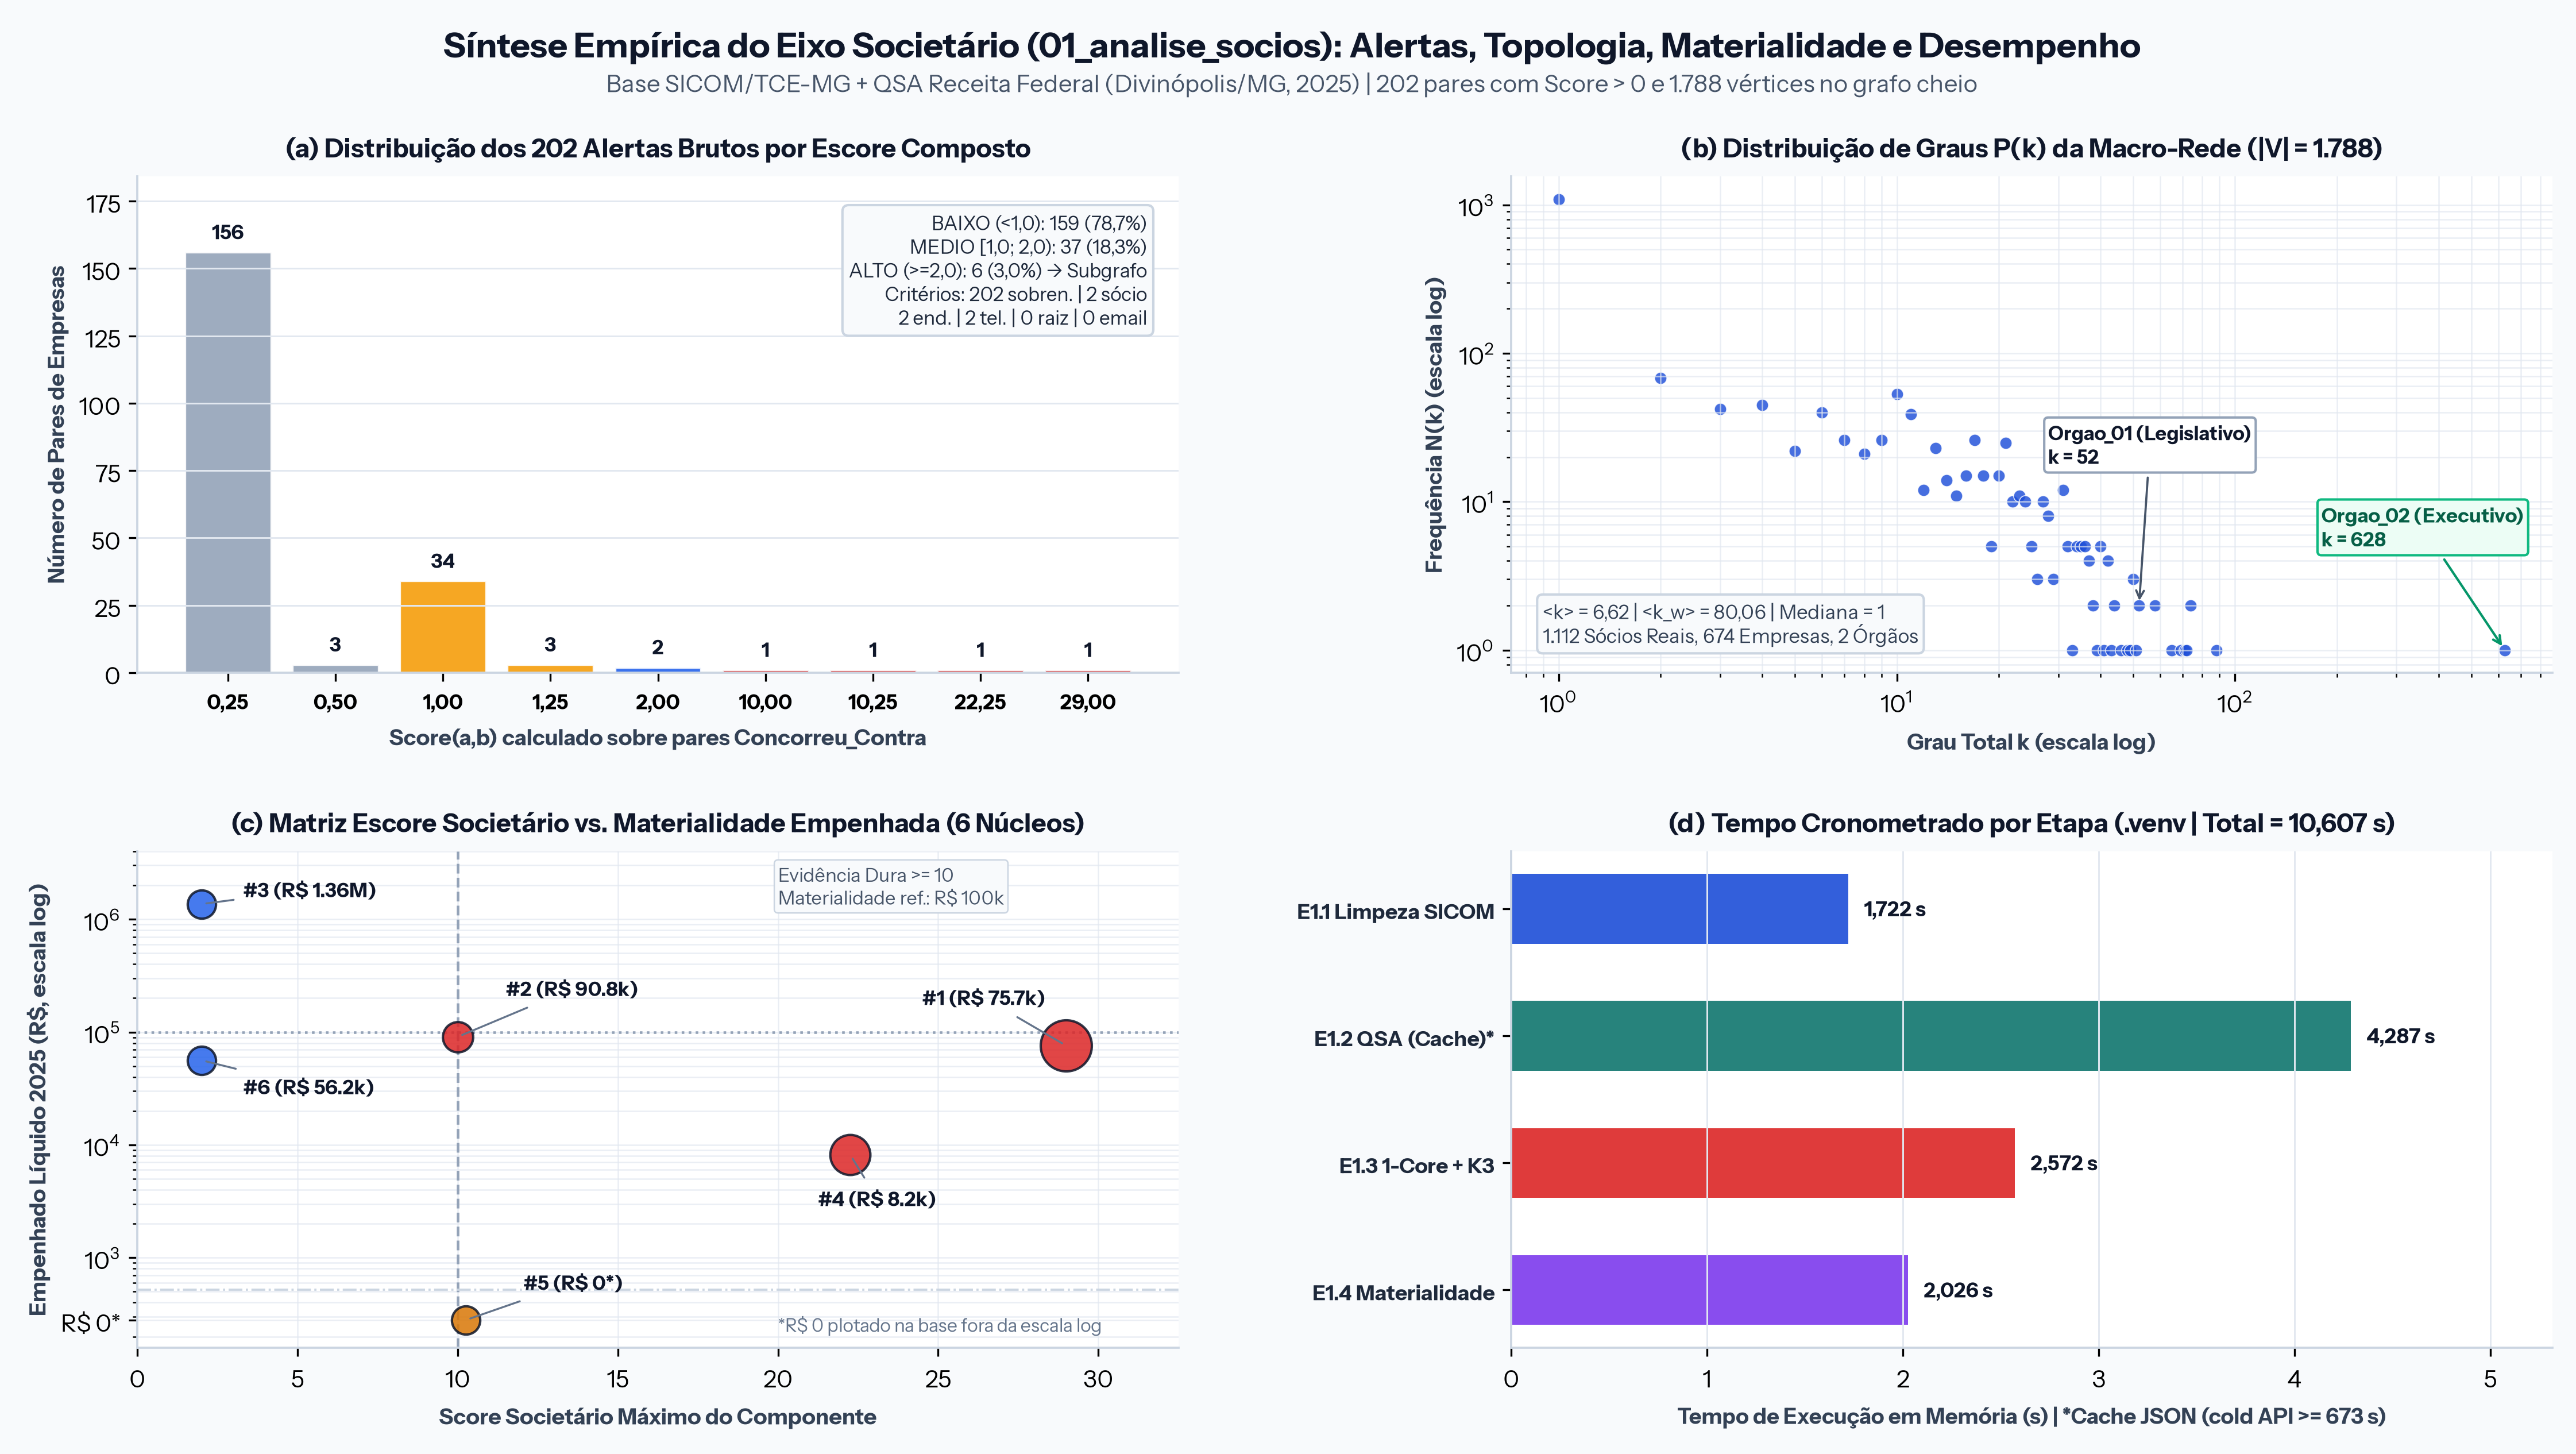
\includegraphics[width=0.71\textwidth]{figures/eixo1_metricas_topologicas.png}
\caption{Painel empírico de síntese do módulo \texttt{01\_\allowbreak analise\_\allowbreak socios}: (a) distribuição dos 202 alertas brutos por escore composto e estratificação \texttt{BAIXO}/\texttt{MEDIO}/\texttt{ALTO}; (b) distribuição de graus $P(k)$ em escala logarítmica da macro-rede ($|V|=1.788$) destacando \texttt{Orgao\_02} e \texttt{Orgao\_01}; (c) matriz \textit{Score} $\times$ Empenhado Líquido separando os núcleos críticos do falso positivo onomástico \#3; e (d) tempos cronometrados das quatro etapas em memória (10,607\,s).}
\label{fig:eixo1_metricas}
\end{figure*}

A inspeção dos seis núcleos agrupados por perfil estrutural na Figura~\ref{fig:eixo1_componentes} evidencia também a distinção comportamental revelada por \texttt{Cert.~/~Itens} e \texttt{Segmento\_\allowbreak Objeto}:
\begin{itemize}
  \item \textbf{Núcleo crítico \#1 ($K_3=1$, $R_{\text{mat}}=325{,}79$, Médico-cirúrgicos):} subgrafo de 5 vértices e 5 arestas conectando \texttt{Emp-1A} e \texttt{Emp-1B} pelo sócio-ponte \texttt{S1*} (fechando um triângulo $K_3$), mesmo endereço (\texttt{End.~A}) e mesmo telefone (\texttt{Tel.~A}, $\text{Score}=29{,}00$), com faturamento ativo em ambas (\texttt{Emp-1A}: R\$\,8.165,00; \texttt{Emp-1B}: R\$\,67.500,00) e atuação no mesmo certame sem sobreposição direta de itens no julgamento (\texttt{1c / 0i});
  \item \textbf{Núcleo crítico \#4 ($2\times K_3$, diamante $K_4-e$, $R_{\text{mat}}=200{,}52$, Odontológicos):} 4 vértices e 5 arestas em que tanto a pessoa jurídica sócia \texttt{PJ S4*} quanto \texttt{S5*} integram simultaneamente o QSA de \texttt{Emp-4A} e \texttt{Emp-4B} ($\text{Score}=22{,}25$). A decomposição \texttt{1c / 59i} confirma competição concentrada item a item em um único pregão (\textbf{60 co-disputas}) com assimetria financeira (\texttt{Emp-4A}: R\$\,0,00; \texttt{Emp-4B}: R\$\,8.200,00 pagos), padrão compatível com \textit{cover bidding} a ser auditado nas atas;
  \item \textbf{Núcleos cadastrais \#2 e \#5 ($\text{Tel.~B}$ e $\text{End.~B}$):} em \#2 (Médicos diversos, \texttt{1c / 0i}), sócios formalmente distintos (\texttt{S6}/\texttt{S7} e \texttt{S8}) compartilham telefone (\texttt{Tel.~B}) e dois sobrenomes raros ($\text{Score}=10{,}00$), somando R\$\,90.760,00 empenhados (R\$\,78.000,00 e R\$\,12.760,00); já \#5 (Equip./Informática, \texttt{1c / 64i}) apresenta padrão compatível com \textit{cover bidding} item a item no mesmo endereço (\texttt{End.~B}, \textbf{65 co-disputas}, $\text{Score}=10{,}25$), porém sem empenho em 2025 ($R_{\text{mat}}=0{,}00$);
  \item \textbf{Triagem onomástica \#3 e \#6 ($P_4$, $\text{Score}=2{,}00$, \texttt{1c / 0i}):} caminhos simples de 4 vértices em Transporte escolar (\#3) e Equipamentos hospitalares (\#6, R\$\,56.250,00 em \texttt{Emp-6B} e R\$\,0,00 em \texttt{Emp-6A}), ligados apenas por dois sobrenomes raros em itens distintos do mesmo certame para revisão manual de homonímia ou parentesco.
\end{itemize}

\subsection{Métricas Gephi, Topologia em Estrela e Desempenho Real}

A Tabela~\ref{tab:eixo1_gephi} compara as métricas topológicas extraídas diretamente dos três arquivos \texttt{.gexf} exportados para o Gephi. Entre a macro-rede (\texttt{grafo\_\allowbreak cheio.gexf}) e os subgrafos reduzidos (\texttt{subgrafos\_\allowbreak fraudes.gexf} e \texttt{subgrafos\_\allowbreak fraudes\_\allowbreak enriquecido.gexf}), a densidade cresce mais de 19 vezes ($0{,}00370 \to 0{,}07077$), o diâmetro da maior componente cai de 7 para 3 e a distância geodésica média reduz-se de $3{,}371$ para $1{,}600$ (\texttt{Comp.~\#1}), mantendo modularidade alta ($Q=0{,}7512$) exatamente alinhada aos 6 componentes de Union-Find. Os valores estruturais de \texttt{subgrafos\_\allowbreak fraudes.gexf} e \texttt{subgrafos\_\allowbreak fraudes\_\allowbreak enriquecido.gexf} coincidem porque a Etapa~4 agrega atributos financeiros e filtros sem alterar a topologia $|V|=26, |E|=23$.

\begin{table}[!t]
\centering
\caption{Tempos reais cronometrados por etapa de \textnormal{\texttt{01\_\allowbreak analise\_\allowbreak socios}} (cache local de 673 CNPJs).}
\label{tab:eixo1_benchmark}
\resizebox{\columnwidth}{!}{%
\begin{tabular}{@{}llcr@{}}
\toprule
\textbf{Etapa / Script} & \textbf{Volume Processado} & \textbf{Complexidade} & \textbf{Tempo (s)} \\
\midrule
E1.1 \texttt{01\_limpeza\_dados.py} & 4 CSVs $\to$ 2.589 nós / 6.652 ar. & $\mathcal{O}(N)$ & 1,722 \\
E1.2 \texttt{02\_enriquecimento\_socios.py} & 673/673 CNPJs (\textit{cache}) $\to$ 1.788 nós / 5.914 ar. & $\mathcal{O}(|E_{\text{conc}}|)$ & 4,287* \\
E1.3 \texttt{03\_reduzir\_grafo.py} & Indução, $1$-Core, Union-Find, $K_3$ $\to$ 26 nós & $\mathcal{O}(|V|+|E|\,d_{\max})$ & 2,572 \\
E1.4 \texttt{04\_materialidade\_financeira.py} & 674 empresas cruzadas + JSON/LGPD & $\mathcal{O}(N)$ & 2,026 \\
\midrule
\textbf{Total em Memória} & \textbf{Pipeline completo (4 etapas)} & -- & \textbf{10,607} \\
\bottomrule
\end{tabular}%
}
\par\vspace{2pt}{\footnotesize *Em execução fria sem \textit{cache}, a BrasilAPI impõe intervalo mínimo $\ge 1{,}0$\,s/CNPJ ($\ge 673$\,s $\approx$ 11,2\,min, $>98{,}4\%$ da latência total).}
\end{table}

Na distribuição de graus da macro-rede (Figura~\ref{fig:eixo1_metricas}b), destaca-se forte assimetria de cauda pesada: enquanto a mediana global vale $k=1$ (sócios vinculados a uma única sociedade), o grau médio é $\langle k \rangle = 6{,}62$ e os dois maiores concentradores pertencem aos órgãos licitantes (\texttt{Orgao\_02} com $k=628$ e força ponderada $k_w=836$; \texttt{Orgao\_01} com $k=52$ e $k_w=53$). Essa topologia gravitacional em estrela comprova a necessidade algorítmica da etapa de indução: se as arestas \textit{Participou\_\allowbreak Licitacao} não fossem removidas antes do Union-Find, os órgãos públicos manteriam praticamente todo o mercado colapsado em uma única componente gigante.

Por fim, a Tabela~\ref{tab:eixo1_benchmark} e a Figura~\ref{fig:eixo1_metricas}~(d) reportam os tempos reais cronometrados em Python (\texttt{-{}-offline} com \textit{cache} JSON): todo o \textit{pipeline} do módulo \texttt{01\_\allowbreak analise\_\allowbreak socios} executou ponta a ponta em \textbf{10,607\,s} (soma exata das quatro etapas), confirmando o comportamento linear e quase linear esperado mesmo após a extração setorial e o cruzamento completo de auditoria. O único gargalo significativo reside na coleta inicial de rede junto à BrasilAPI, que impõe ao menos 673\,s (11\,min\,13\,s) para os 673 CNPJs válidos devido ao limite de 1 requisição/segundo — tornando o \textit{cache} incremental em disco essencial para auditoria interativa e escalabilidade operacional.

\section{Conclusão e Trabalhos Futuros}
\label{sec:conclusao}


Este trabalho apresentou uma abordagem algorítmica e topológica, baseada em grafos heterogêneos multicamada, para a identificação de indícios de conluio e simulação de competitividade em contratações públicas municipais. A aplicação aos dados abertos do SICOM/TCE-MG, referentes ao exercício de 2025 do município de Divinópolis/MG, demonstrou o potencial da integração entre registros licitatórios, informações cadastrais da Receita Federal, obtidas por meio da BrasilAPI, e técnicas de análise estrutural para identificar relações que não são evidentes em consultas isoladas às bases de dados.

As principais contribuições do estudo podem ser sintetizadas em três aspectos.

\subsection{Eficiência da Redução Topológica}

A combinação entre a filtragem por escore multidimensional ($\theta \geq 2{,}00$), a remoção de vértices isolados e a identificação de componentes conexas permitiu reduzir a rede original, composta por 1.788 vértices e 5.914 arestas, a um subgrafo de interesse pericial com apenas 26 vértices e 23 arestas. Essa transformação corresponde a uma redução de 98,55\% no número de vértices e de 99,61\% no número de arestas.

O procedimento permitiu eliminar elementos sem participação nas relações selecionadas, reduzindo a interferência da estrutura geral da rede e concentrando a análise em seis componentes conexas prioritárias para auditoria. Dessa forma, a metodologia demonstrou que a redução estrutural determinística pode tornar redes de contratações públicas mais interpretáveis, preservando as relações consideradas relevantes segundo os critérios de pontuação estabelecidos.

\subsection{Identificação de Indícios de Controle e Vínculos Compartilhados}

A incorporação de informações do Quadro de Sócios e Administradores (QSA), combinada à análise de relações societárias e à identificação de motivos estruturais, permitiu localizar três motivos triangulares na representação utilizada para a análise, distribuídos em dois núcleos críticos. Entre os casos identificados, destaca-se a ocorrência de relações societárias compartilhadas envolvendo sócio pessoa física e uma holding controladora, associadas à disputa simultânea de 59 itens em um mesmo certame.

Além das coincidências societárias, a ponderação onomástica inspirada no princípio IDF e a normalização de endereços e telefones permitiram identificar quatro núcleos adicionais sem coincidência formal de sócios no QSA. Esses resultados evidenciam a utilidade da combinação de diferentes atributos cadastrais e relacionais para a identificação de possíveis vínculos domiciliares, operacionais e familiares que poderiam não ser detectados por cruzamentos cadastrais convencionais.

\subsection{Contribuição ao Controle Externo}

O pipeline desenvolvido constitui uma ferramenta de apoio à triagem de procedimentos licitatórios, oferecendo critérios explícitos de pontuação, relações rastreáveis e resultados passíveis de inspeção. Diferentemente de abordagens baseadas exclusivamente em modelos opacos, a metodologia permite relacionar os indícios identificados aos atributos e às conexões que contribuíram para sua classificação.

Ressalta-se, contudo, que os resultados possuem caráter indiciário. A identificação de relações societárias, cadastrais ou estruturais não constitui, isoladamente, comprovação de conluio ou de irregularidade. Os resultados devem, portanto, orientar procedimentos posteriores de auditoria e investigação, com verificação documental e análise contextual pelos órgãos competentes. A utilização de identificadores pseudonimizados também foi considerada na arquitetura, em alinhamento com os princípios de proteção de dados estabelecidos pela Lei Geral de Proteção de Dados Pessoais (Lei nº 13.709/2018).

\subsection{Trabalhos Futuros}

Como continuidade desta pesquisa, identificam-se três direções principais. A primeira consiste na incorporação de atributos temporais e financeiros das propostas comerciais e dos lances registrados nas atas de julgamento, especialmente nos dados de \texttt{julgLicitacao.csv}. Essa extensão permitiria investigar padrões de alternância de vencedores (\textit{bid rotation}) e apresentação de propostas de cobertura (\textit{cover bidding}), ampliando a análise para além das relações cadastrais e societárias.

A segunda direção consiste na integração de métricas de centralidade e algoritmos de detecção de comunidades em bases plurianuais do SICOM. Essa abordagem possibilitaria acompanhar a evolução temporal dos grupos econômicos, identificar mudanças nas relações entre fornecedores e órgãos contratantes e investigar a persistência de padrões suspeitos ao longo de diferentes exercícios financeiros.

Por fim, pretende-se investigar a aplicação de modelos de aprendizado de representação em grafos heterogêneos (\textit{Heterogeneous Graph Neural Networks}), com o objetivo de explorar mecanismos de calibração dos pesos do escore multidimensional a partir de conjuntos históricos de casos analisados ou julgados pelos órgãos de controle. Essa possibilidade deverá ser avaliada considerando a disponibilidade de dados rotulados, a interpretabilidade dos modelos e a necessidade de preservar a rastreabilidade dos critérios utilizados na identificação dos indícios.


% =============================================================================
% REFERÊNCIAS BIBLIOGRÁFICAS
% =============================================================================
\bibliographystyle{IEEEtran}
\bibliography{references}

\end{document}
